\documentclass[11pt]{article}
\usepackage[utf8]{inputenc}
\usepackage[T1]{fontenc}
\usepackage{lmodern}
\usepackage[margin=1in]{geometry}
\usepackage{graphicx}
\usepackage{booktabs}
\usepackage{longtable}
\usepackage{array}
\usepackage{amssymb}
\usepackage{amsmath}
\usepackage[font=small]{caption}
\usepackage{microtype}
\usepackage{setspace}
\usepackage[hidelinks]{hyperref}
\graphicspath{{figures/}}
\setlength{\parskip}{0.6em}
\setlength{\parindent}{0pt}
\title{"Like, Literally, Love": A Lexical Analysis of Vocabulary Complexity in \emph{Love Island USA} Season 4}
\author{[Your Name]\\[2pt]\small Course / Institution: [If applicable]}
\date{June 2026}
\begin{document}
\maketitle
\begin{abstract}

This paper investigates the lexical characteristics of reality television discourse through a corpus-based analysis of \emph{Love Island USA} Season 4 (2022). Drawing on the subtitle transcripts of all 38 episodes --- a 224,815-token corpus of on-screen speech, including contestant dialogue, host narration, and voiceover --- we examine vocabulary richness, word frequency distributions, filler word usage, part-of-speech patterns, and sentiment across the season. Our findings indicate that the show exhibits a narrow active vocabulary dominated by a small set of high-frequency words: the 100 most frequent word types account for 61\% of all tokens, and word frequency follows Zipf's Law almost exactly (log-log slope = $-$1.45, R\textsuperscript{2} = 0.98). A corpus Type-Token Ratio of 0.035 and a mean per-episode MTLD of 59.96 indicate low lexical diversity relative to benchmarks for spontaneous speech ($\approx$72; McCarthy \& Jarvis, 2010). Diversity shows no significant trend across the season (MTLD vs. episode: r = $-$0.11, p = .52). The discourse is highly subjective (mean subjectivity = 0.56) and uniformly positive in polarity, yet conveyed through a strikingly limited adjectival vocabulary (8.4\% of tokens). These results have implications for understanding how media consumption shapes language exposure and, potentially, language development in audiences.

\end{abstract}
\smallskip\noindent\textbf{Keywords:} lexical diversity, reality television, corpus linguistics, spoken language, vocabulary richness, \emph{Love Island}


\section*{1. Introduction}

Reality television has become one of the dominant media formats of the twenty-first century, attracting hundreds of millions of viewers worldwide. Among these programs, \emph{Love Island} --- originally a British format, now franchised internationally --- is particularly notable for its unscripted, conversational nature. Contestants are placed in a villa and filmed continuously, generating hours of spontaneous dialogue per episode.

Unlike scripted television, in which writers carefully craft dialogue to serve narrative and character goals, reality TV captures speech as it naturally occurs among a specific demographic. This raises an important question: how linguistically rich is the language produced in this environment?

The present study is motivated by a widely cited observation in applied linguistics: while the English language contains approximately 170,000 words in current use (Oxford English Dictionary), the average adult speaker actively uses somewhere between 20,000 and 35,000 words, and comfortable everyday communication typically requires only around 3,000 high-frequency words (Nation, 2001). If everyday conversation concentrates in such a narrow vocabulary range, it follows that informal, unscripted television content may do the same --- or may do so even more acutely, given the emotional, social, and performative pressures contestants face.

This paper asks: \emph{How lexically diverse is the language used in Love Island USA Season 4, and what patterns of vocabulary use emerge across the season?}

\subsection*{1.1 Research Questions}

\par\noindent 1. What is the overall vocabulary richness of \emph{Love Island USA} Season 4, as measured by Type-Token Ratio (TTR), Root TTR, and MTLD?
\par\noindent 2. Which words dominate the discourse, and how concentrated is word usage around a small high-frequency core?
\par\noindent 3. What role do filler and hedge words play in contestant speech?
\par\noindent 4. What is the part-of-speech profile of the corpus, and what does it reveal about the grammatical complexity of the language?
\par\noindent 5. How does sentiment vary across episodes, and does it correlate with narrative arc?


\section*{2. Literature Review}

\subsection*{2.1 Lexical Diversity and Its Measurement}

Lexical diversity --- the range and variety of vocabulary used in a text or speech sample --- is a core concept in corpus linguistics and language assessment. Early measures such as the Type-Token Ratio (TTR), which divides the number of unique word types by the total number of tokens, provided an intuitive index of vocabulary richness but were found to be highly sensitive to text length (Richards, 1987). Longer texts naturally accumulate more repetitions, artificially lowering TTR.

To address this, researchers developed length-normalised measures. Root TTR (RTTR) partially corrects for length by dividing unique types by the square root of total tokens. More sophisticated measures include the Measure of Textual Lexical Diversity (MTLD; McCarthy \& Jarvis, 2010), which calculates the mean length of sequential word strings maintaining a TTR above a threshold (0.72), making it robust to text length variation.

For reference, spoken language MTLD scores typically range from 60 to 100, while literary texts often exceed 100 (McCarthy \& Jarvis, 2010).

\subsection*{2.2 Vocabulary in Spoken vs. Written Discourse}

Spoken language is consistently found to be lexically simpler than written language across multiple dimensions: shorter words, higher proportions of pronouns and function words, and greater reliance on a small core of high-frequency vocabulary (Biber et al., 1999). Informal conversation, in particular, is characterised by a heavy reliance on what Leech (2000) called "the top hundred" high-frequency words, which can account for over 50\% of all tokens in casual speech corpora.

\subsection*{2.3 Language in Reality Television}

The linguistic analysis of reality television is a relatively recent field. Thornborrow and Morris (2004) examined \emph{Big Brother} (UK) and found that contestant speech displays features of both private conversation and performative public speech, given that contestants are always aware of cameras. This awareness may constrain lexical choice, favouring safe, broadly comprehensible language.

Fleiss (2018) noted that reality television contestants frequently use hedging and vague language devices --- words such as \emph{like}, \emph{literally}, \emph{basically}, and \emph{kind of} --- as sociolinguistic signals of solidarity and informality. These devices, sometimes called "approximators" (Channell, 1994), serve relational rather than referential functions.

To date, no published study has examined the lexical properties of \emph{Love Island USA} specifically. This paper begins to fill that gap.


\section*{3. Methodology}

\subsection*{3.1 Data Collection}

The corpus consists of transcripts from all 38 episodes of \emph{Love Island USA} Season 4 (originally aired July--August 2022 on Peacock), sourced from Subslikescript.com. Transcripts were scraped programmatically using Selenium and Chrome WebDriver to navigate the site's bot-protection system, and stored in a structured CSV file containing episode number, title, word count, and full transcript text.

The total corpus comprises \textbf{224,815} word tokens (after preprocessing) across all \textbf{38} episodes; all episodes exceeded the 50-word threshold used to screen out failed scrapes.

\textbf{Scope of the corpus.} The source material is closed-caption subtitle text, which records \emph{all} on-screen speech without speaker attribution. The corpus therefore conflates three voices: contestant dialogue (the large majority), host/narrator commentary (e.g., the season's voiceover and presenter links), and occasional on-screen song lyrics. Because the transcripts are not speaker-diarised, these voices cannot be reliably separated automatically. We therefore frame the analysis as a study of \emph{Love Island USA} spoken discourse as broadcast, rather than of contestant idiolect specifically. This is revisited in the Limitations.

\subsection*{3.2 Text Preprocessing}

Raw transcript text was cleaned through the following pipeline:

\par\noindent 1. Removal of subtitle speaker-change dashes (leading "- ") and metadata tags (e.g., \texttt{[FAILED]}, URLs)
\par\noindent 2. Lowercasing
\par\noindent 3. Removal of non-alphabetic characters (retaining apostrophes for contractions)
\par\noindent 4. Tokenisation using the NLTK \texttt{word\_tokenize} function
\par\noindent 5. Removal of single-character tokens

Step 5 means the single-letter words \emph{I} and \emph{a} are excluded from all token-level counts; reported frequencies and ratios should be read with this in mind. Sentence segmentation for the words-per-sentence statistic was performed on the \emph{raw} (pre-cleaning) text, since lowercasing and punctuation removal destroy sentence boundaries.

Stopword removal (using NLTK's English stopword list) was applied selectively --- retained for frequency and POS analysis, removed for content word and word cloud analysis.

\subsection*{3.3 Analytical Measures}

The following analyses were conducted using Python (v3.12) with the libraries \texttt{nltk}, \texttt{textblob}, \texttt{wordcloud}, \texttt{pandas}, \texttt{numpy}, \texttt{scipy}, \texttt{matplotlib}, and \texttt{seaborn}:

\begin{longtable}{p{0.237\linewidth}p{0.683\linewidth}}
\toprule
Analysis & Method \\
\midrule
\endfirsthead
\toprule
Analysis & Method \\
\midrule
\endhead
\bottomrule
\endlastfoot
Lexical diversity & TTR, Root TTR, MTLD per episode \\
Word frequency & Counter-based frequency ranking; cumulative top-\emph{N} coverage \\
Zipf's Law & OLS regression of log\textsubscript{10}(frequency) on log\textsubscript{10}(rank) \\
Filler word usage & Targeted frequency count against a 24-item predefined list \\
Part-of-speech distribution & Penn Treebank POS tagging (NLTK averaged perceptron), 50,000-token sample \\
Sentiment & TextBlob polarity ($-$1 to +1) and subjectivity (0 to 1), full episode text \\
Across-season trends & Pearson and Spearman correlation of diversity/sentiment against episode number \\
Word length & Character-length distribution of all tokens \\
Vocabulary growth & Cumulative type count against cumulative token count \\
\end{longtable}


\section*{4. Results}

\subsection*{4.1 Corpus Overview}

The Season 4 corpus contains a total of \textbf{224,815} word tokens, of which \textbf{7,856} are unique word types. Table 1 presents the key summary statistics, separating corpus-level measures from per-episode means (the latter averaged across the 38 episodes).

\textbf{Table 1. Summary Statistics --- Love Island USA Season 4 Corpus}

\begin{longtable}{p{0.85\linewidth}l}
\toprule
Metric & Value \\
\midrule
\endfirsthead
\toprule
Metric & Value \\
\midrule
\endhead
\bottomrule
\endlastfoot
Total episodes & 38 \\
Total word tokens & 224,815 \\
Unique word types & 7,856 \\
Type-Token Ratio (TTR), whole corpus & 0.035 \\
Root TTR, whole corpus & 16.57 \\
Mean per-episode TTR & 0.179 \\
Mean per-episode Root TTR & 13.54 \\
Mean per-episode MTLD & 59.96 \\
Mean word length (chars) & 4.03 \\
Total sentences (est.) & 36,758 \\
Mean words per sentence & 6.1 \\
\end{longtable}

The whole-corpus TTR (0.035) is far lower than any per-episode TTR because TTR falls mechanically as token count grows; the length-robust MTLD is therefore the more interpretable diversity measure and is used for cross-text comparison below.

\subsection*{4.2 Word Frequency Distribution}

Figure 1 presents the 50 most frequent words in the corpus. As expected of informal spoken discourse, the list is dominated by function words and pronouns. The ten most frequent tokens, in order, are \emph{you}, \emph{to}, \emph{like}, \emph{the}, \emph{and}, \emph{it}, \emph{that}, \emph{know}, \emph{yeah}, and \emph{do}. (The single-letter pronoun \emph{I} is absent only because single-character tokens were removed in preprocessing; it would otherwise rank first.)

\begin{figure}[h]
\centering
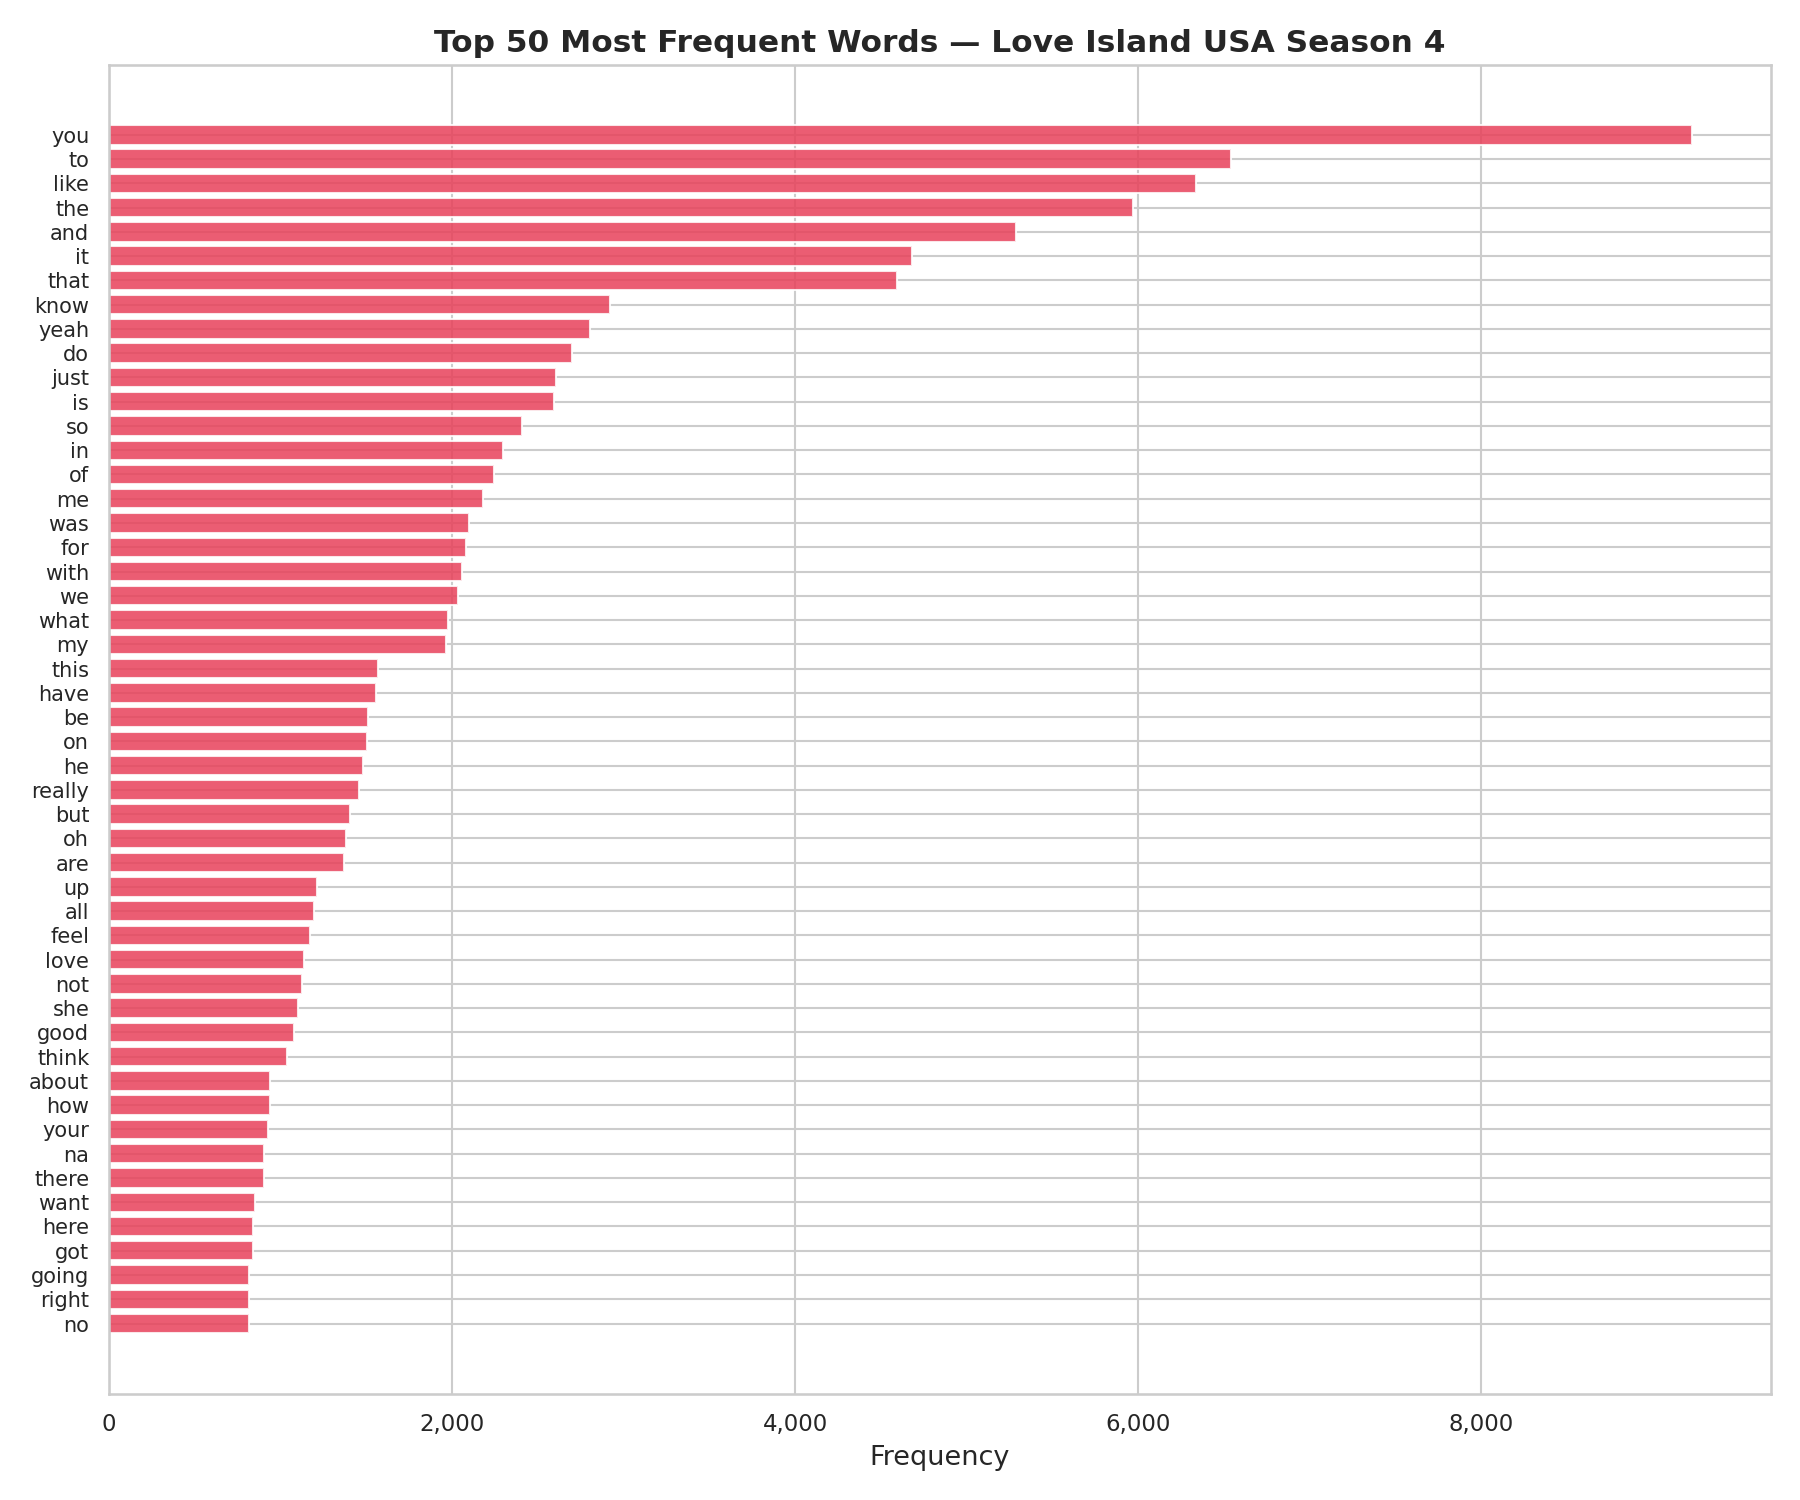
\includegraphics[width=\linewidth]{01_top50_words.png}
\caption*{\textbf{Figure 1.} Top 50 Most Frequent Words}
\end{figure}

The top 10 words alone account for \textbf{22.7\%} of all tokens, the top 50 for \textbf{48.7\%}, and the top 100 for \textbf{61.0\%}; just 1,000 word types (about 13\% of the vocabulary) cover \textbf{91.1\%} of the entire corpus. This extreme concentration is consistent with Zipf's Law: an OLS regression of log\textsubscript{10}(frequency) on log\textsubscript{10}(rank) yields a slope of \textbf{$-$1.45} with \textbf{R\textsuperscript{2} = 0.98} (p $<$ .001), confirming the near-linear rank--frequency relationship visible in the log-log plot (Figure 2).

\begin{figure}[h]
\centering
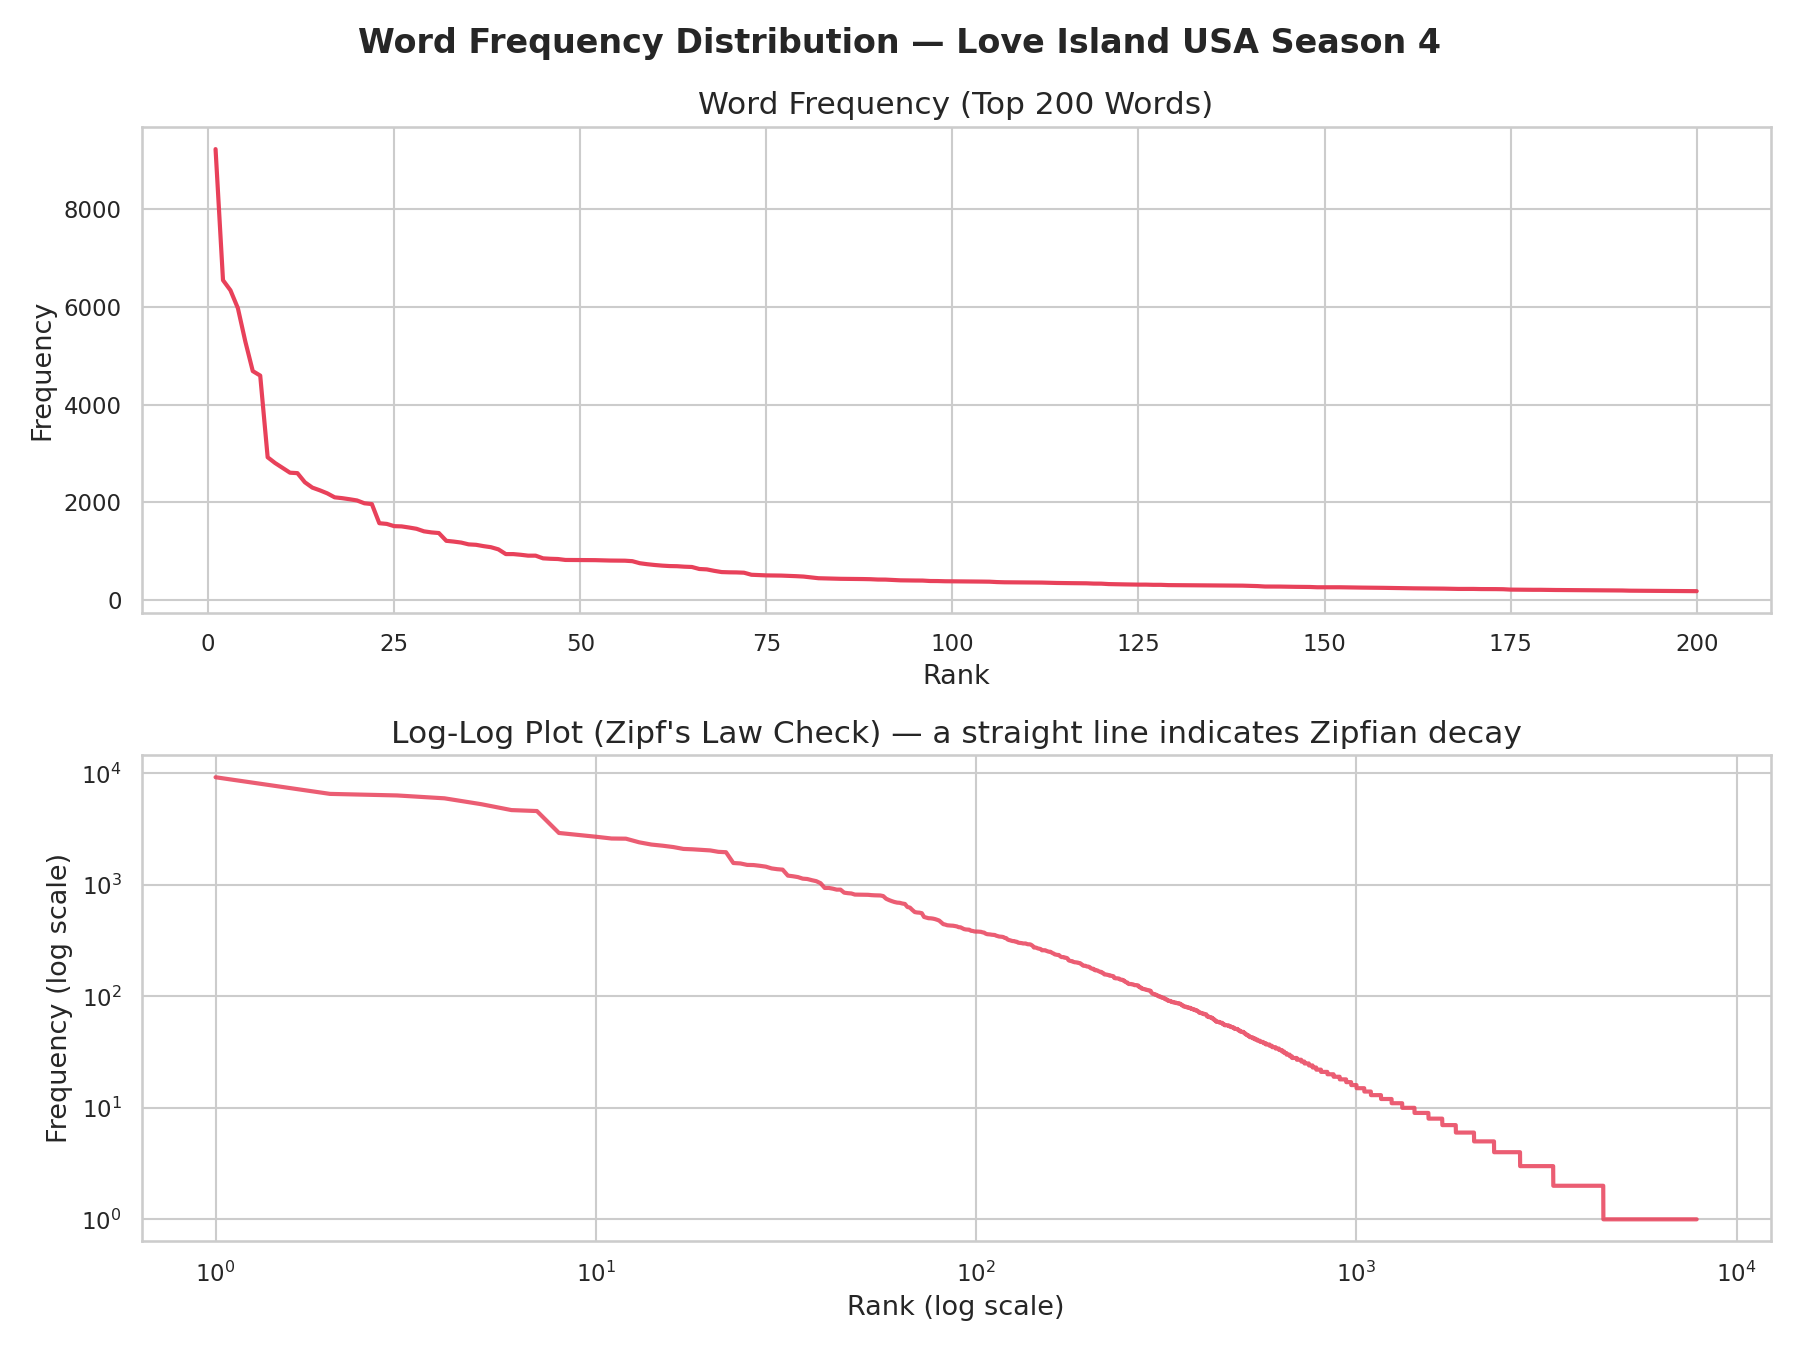
\includegraphics[width=\linewidth]{02_word_frequency_distribution.png}
\caption*{\textbf{Figure 2.} Word Frequency Distribution and Zipf's Law Check}
\end{figure}

Notably, the word \emph{like} appears \textbf{6,338} times (\textbf{28.2} per 1,000 words) --- the most frequent content-bearing word and the third most frequent token overall. It functions both as a comparative/preposition and, predominantly, as a discourse marker and quotative ("I was like\ldots{}") --- a characteristic feature of American informal speech.

\subsection*{4.3 Lexical Diversity}

Figure 3 displays TTR, Root TTR, and MTLD scores across all 38 episodes. Episode-level TTR ranges from 0.125 (Episode 38) to 0.245 (Episode 30), with a mean of 0.179. MTLD scores range from 40.42 (Episode 36) to 81.93 (Episode 5), with a mean of 59.96.

\begin{figure}[h]
\centering
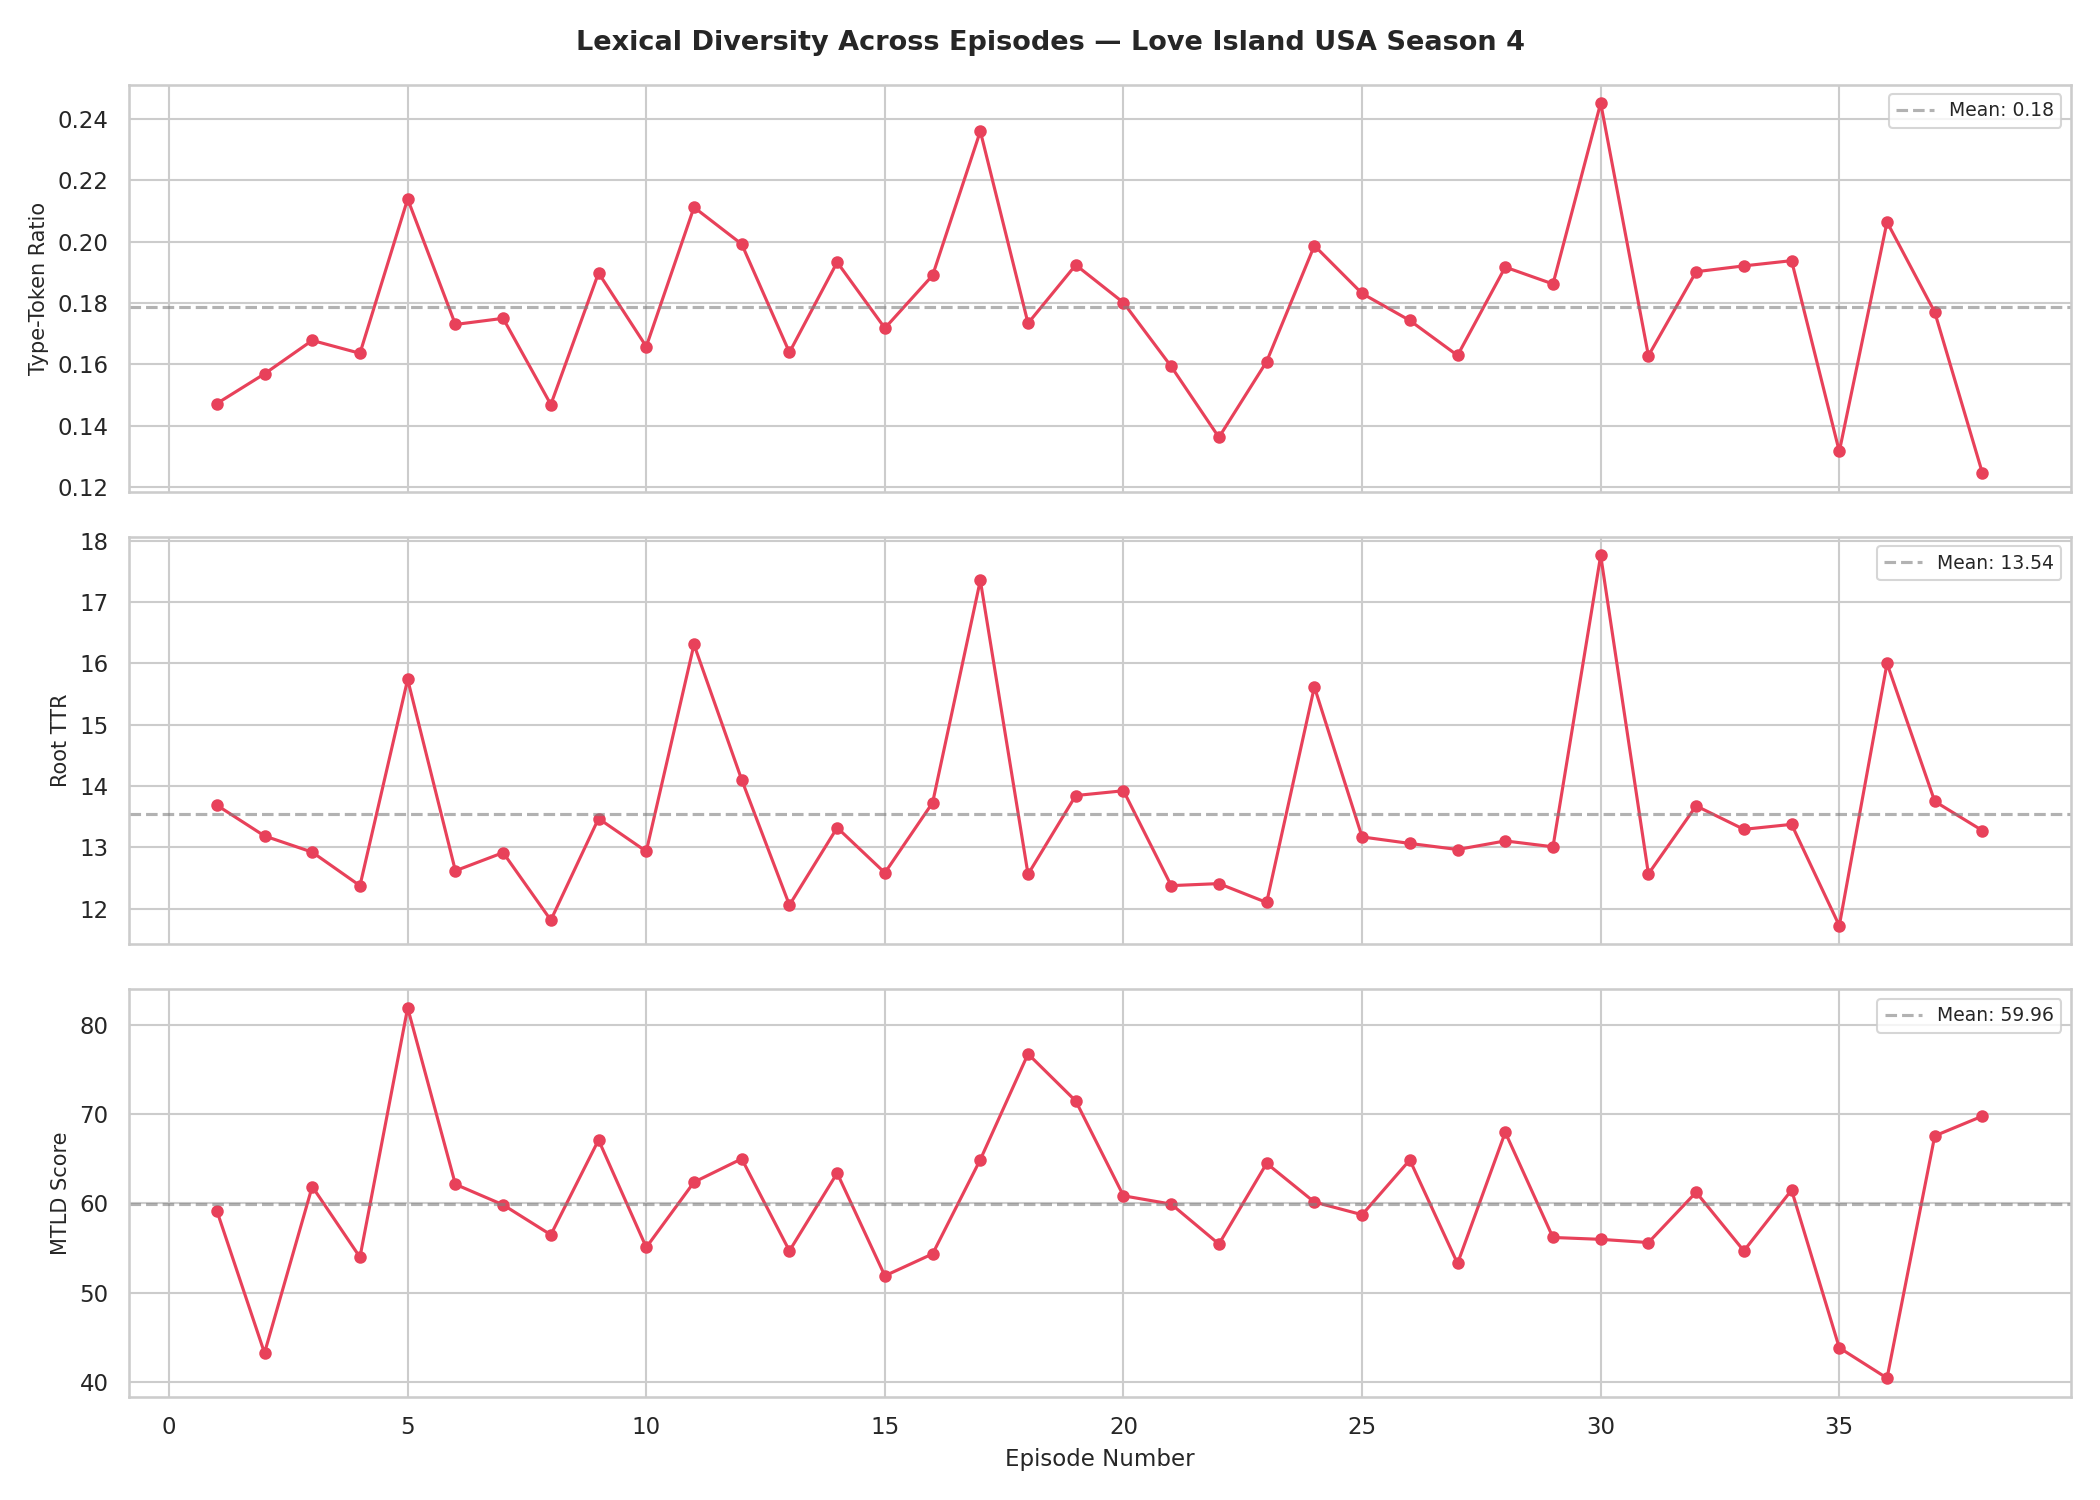
\includegraphics[width=\linewidth]{03_lexical_diversity_per_episode.png}
\caption*{\textbf{Figure 3.} Lexical Diversity Across Episodes}
\end{figure}

These scores suggest low lexical diversity relative to established benchmarks. For context, McCarthy and Jarvis (2010) report mean MTLD scores of approximately 72 for spontaneous speech; the present corpus yields a mean of 59.96, which is below this benchmark --- i.e., the discourse is \emph{less} lexically varied than ordinary spontaneous conversation.

No statistically significant trend was observed across the season for any diversity measure (MTLD vs. episode: Pearson r = $-$0.11, p = .52; TTR vs. episode: r = 0.05, p = .78). Vocabulary richness therefore does not systematically increase or decrease as the competition progresses; the episode-to-episode fluctuation in Figure 3 is largely attributable to differences in episode length and content (e.g., longer recap or finale episodes) rather than a directional shift.

\subsection*{4.4 Vocabulary Profiles: Word Clouds}

Figures 4 and 5 present word clouds of the full corpus and content words respectively. The full-corpus cloud (Figure 4) is visually dominated by pronouns and function words, reflecting the heavily interpersonal nature of the discourse.

\begin{figure}[h]
\centering
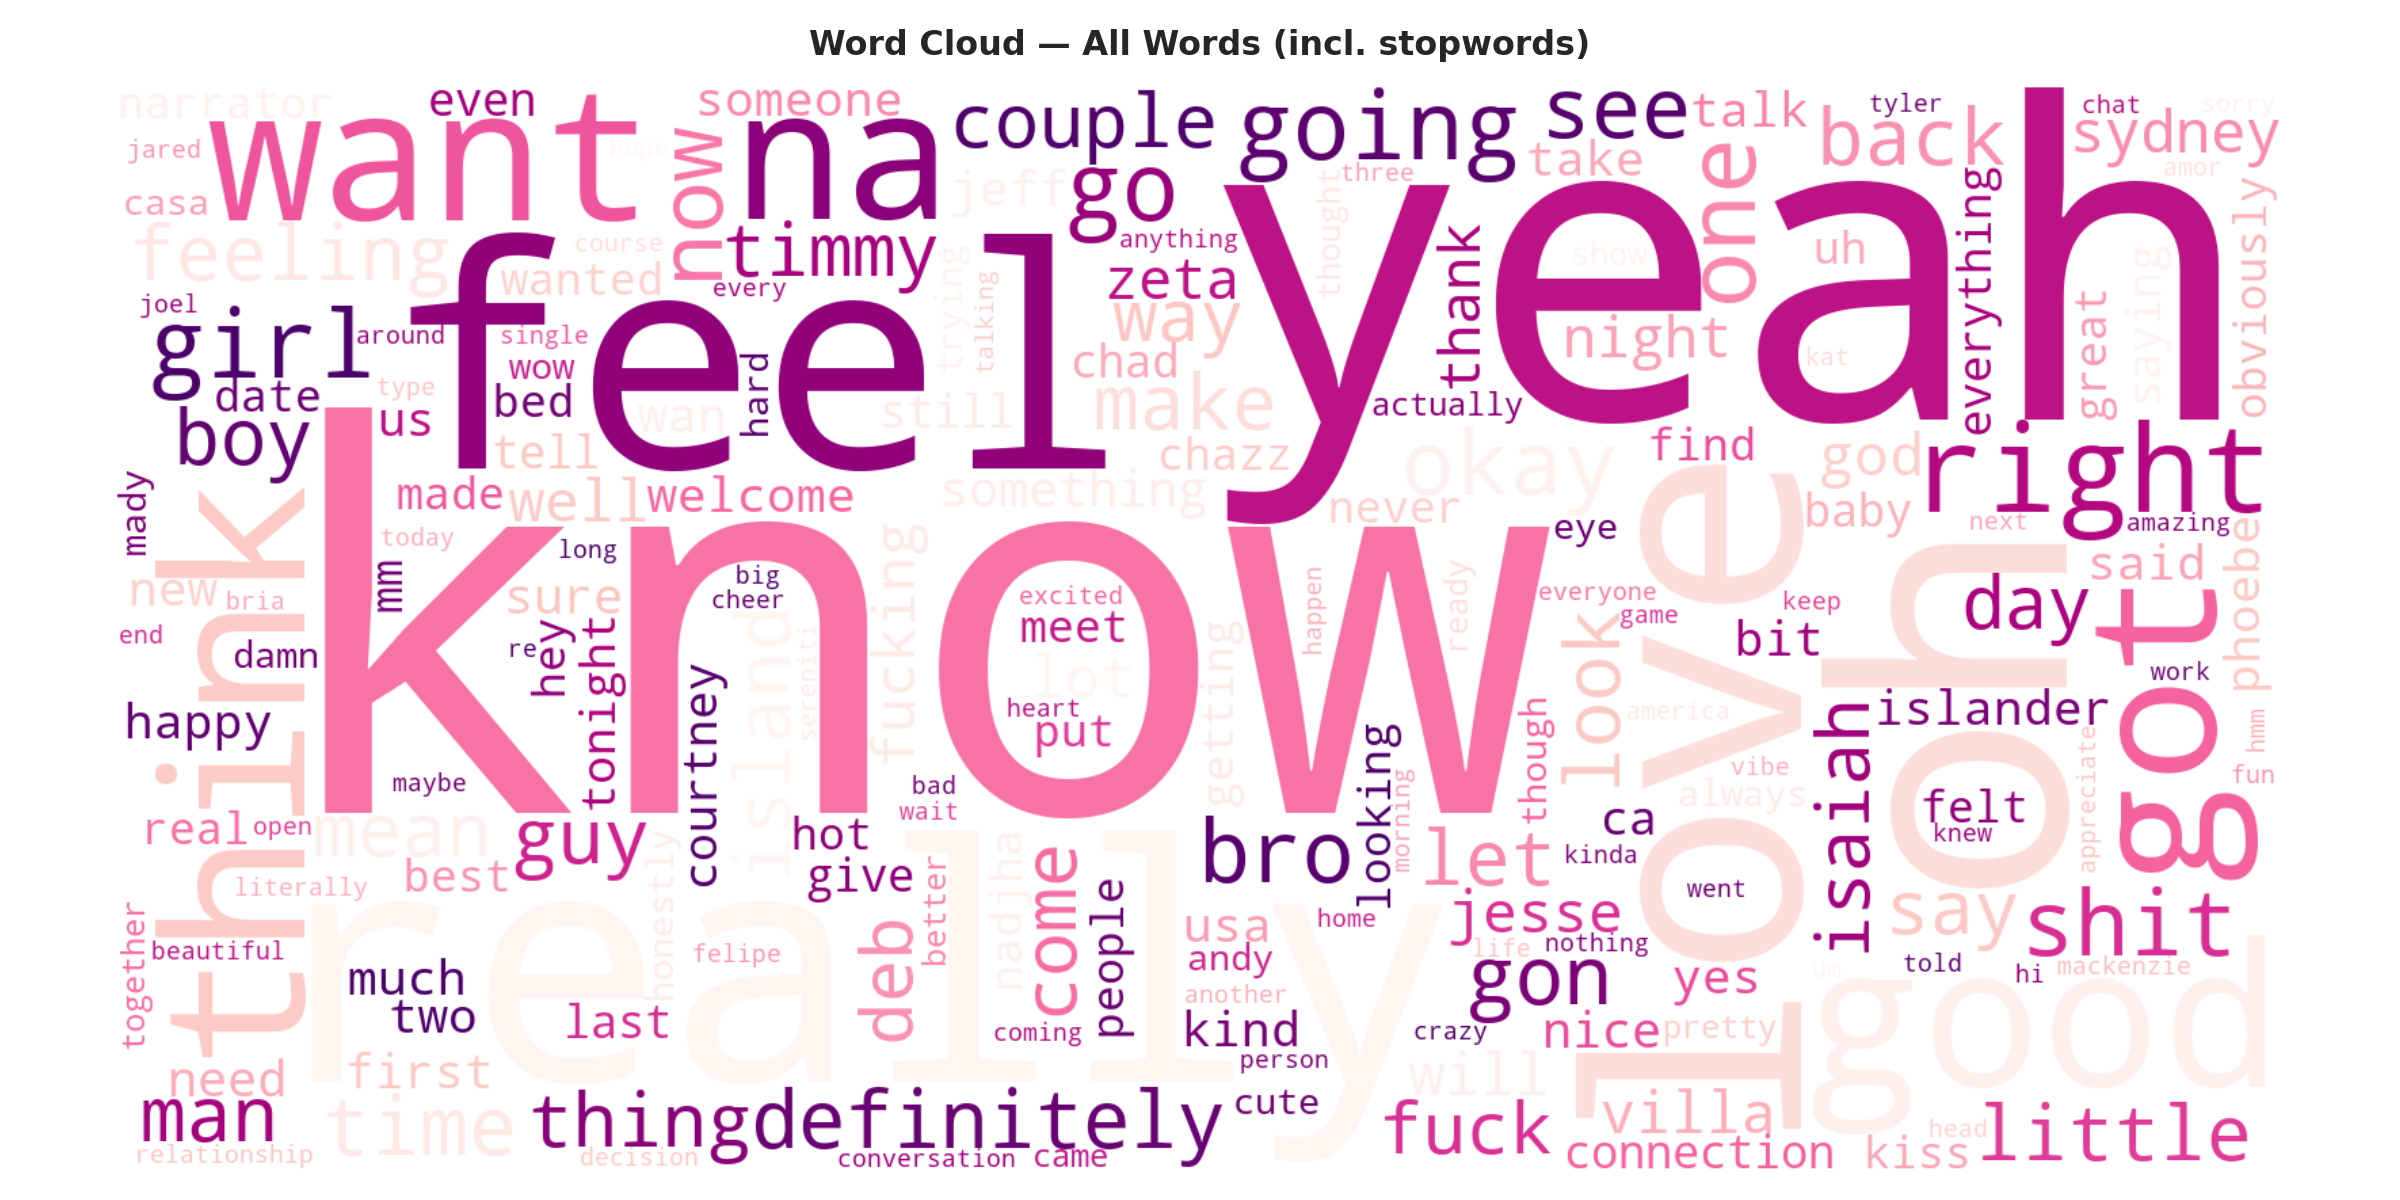
\includegraphics[width=\linewidth]{04_wordcloud_all.png}
\caption*{\textbf{Figure 4.} Word Cloud --- All Words}
\end{figure}

\begin{figure}[h]
\centering
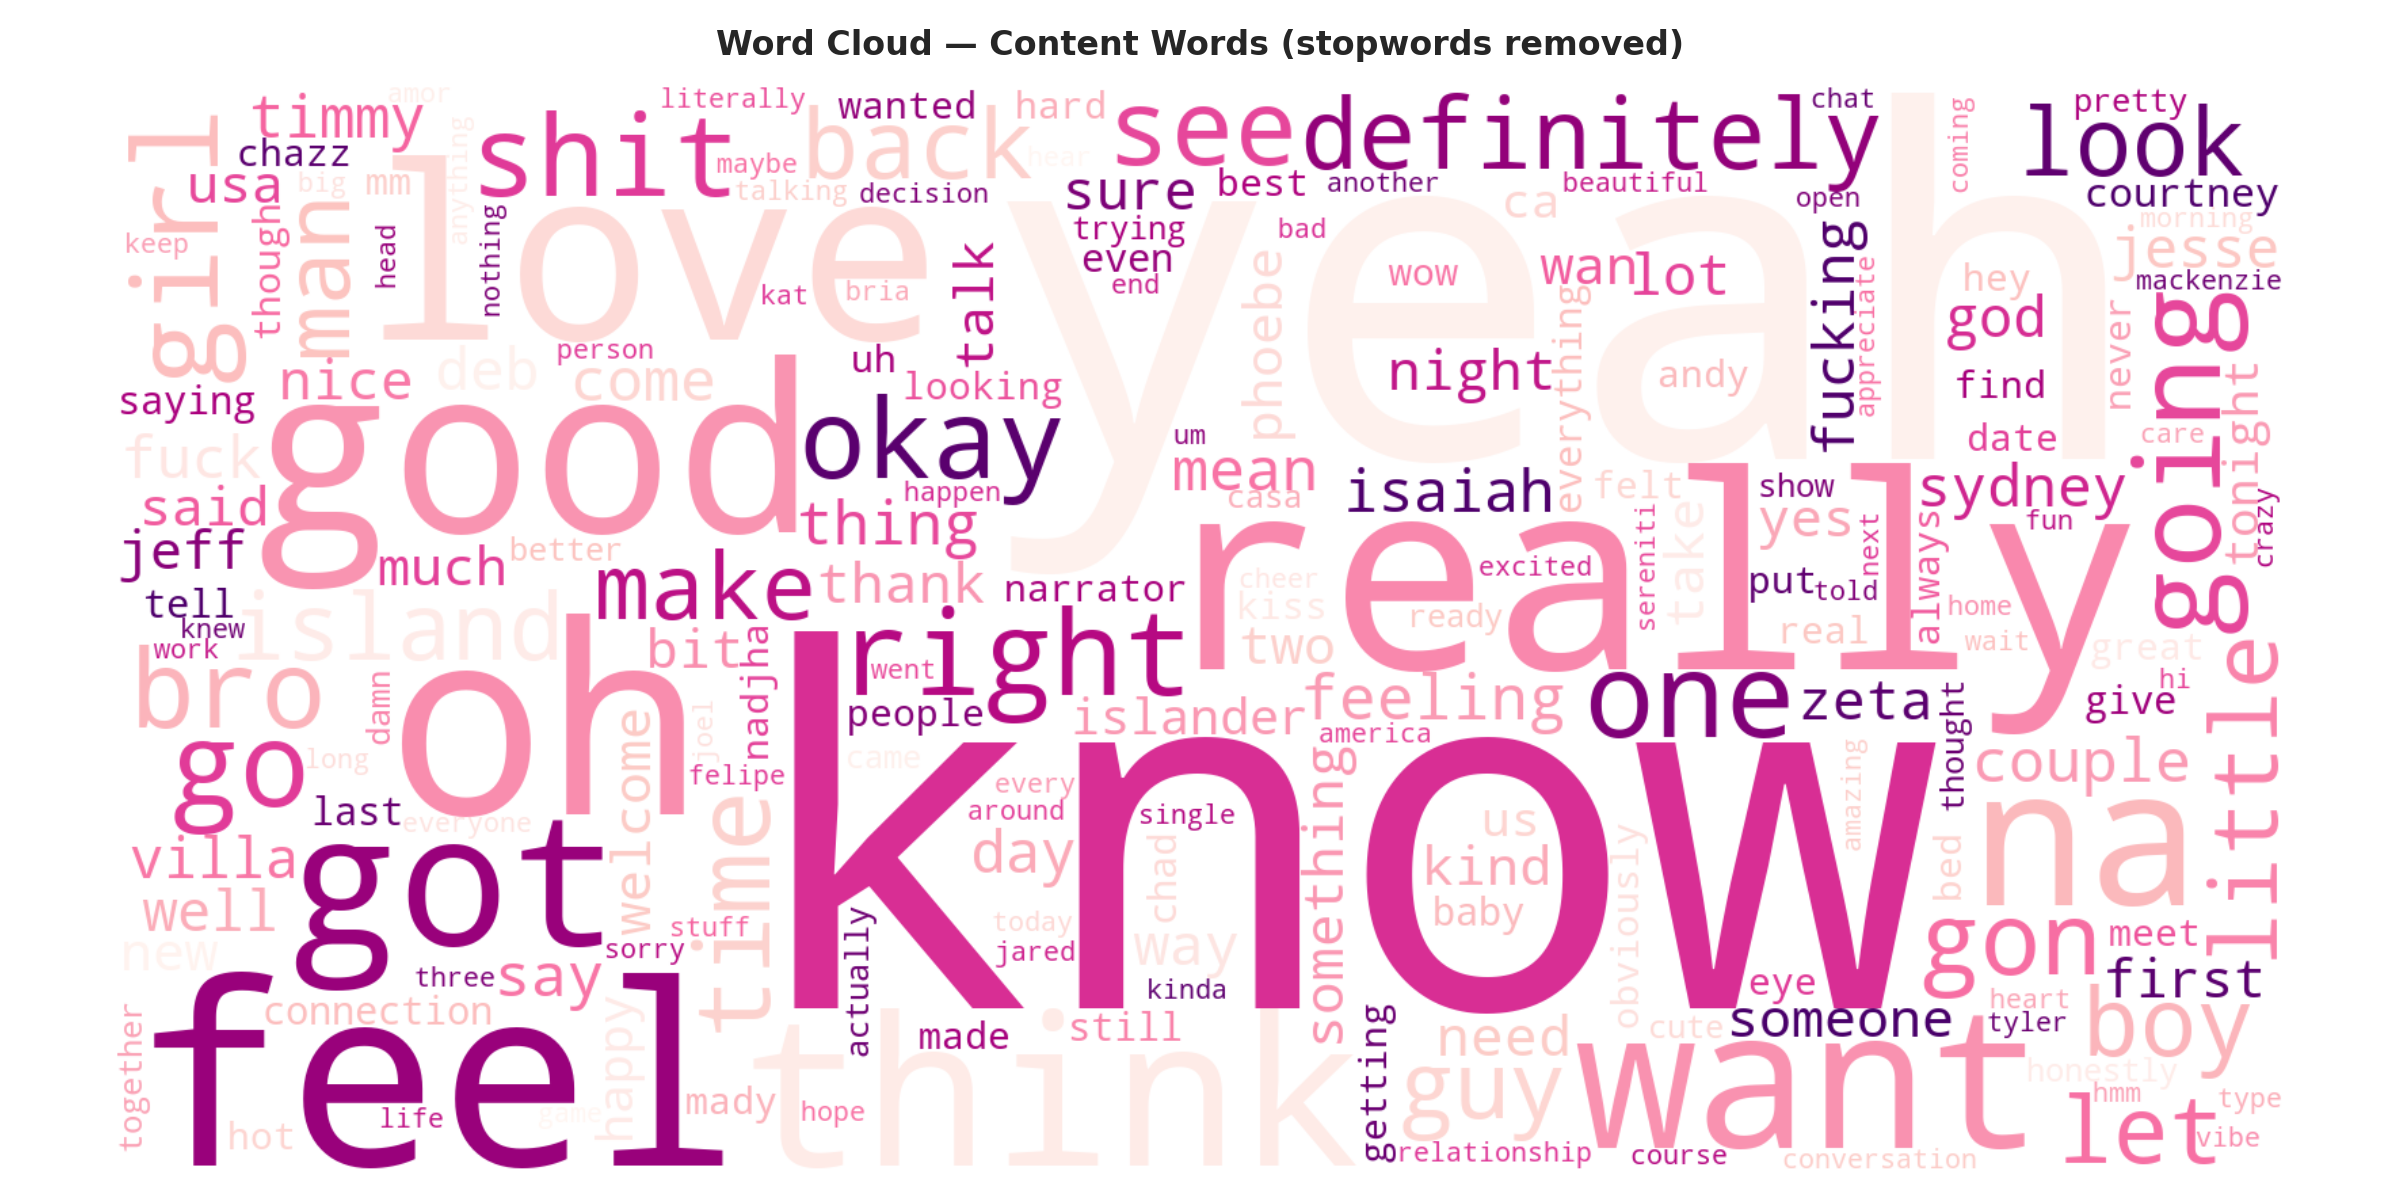
\includegraphics[width=\linewidth]{05_wordcloud_no_stopwords.png}
\caption*{\textbf{Figure 5.} Word Cloud --- Content Words Only (stopwords removed)}
\end{figure}

With stopwords removed (Figure 5), the content word profile reveals a cluster of emotionally and relationally focused vocabulary. After discourse markers (\emph{like}, \emph{know}, \emph{yeah}, \emph{really}, \emph{oh}), the most frequent content words are \emph{feel}, \emph{love}, \emph{good}, \emph{think}, \emph{want}, \emph{going}, \emph{get}, and \emph{time}. This emotion- and volition-oriented lexicon (\emph{feel}, \emph{love}, \emph{want}, \emph{think}) is consistent with the show's thematic focus on romantic connection and self-presentation.

\subsection*{4.5 Filler and Hedge Word Usage}

Figure 6 presents the frequency of pre-defined filler and hedge words per 1,000 tokens. The most frequent are \emph{like} (28.2 per 1,000 words), \emph{know} (13.0), and \emph{yeah} (12.5), followed by \emph{just} (11.6) and \emph{really} (6.5). \emph{Like} alone is more than twice as frequent as any other item on the list.

\begin{figure}[h]
\centering
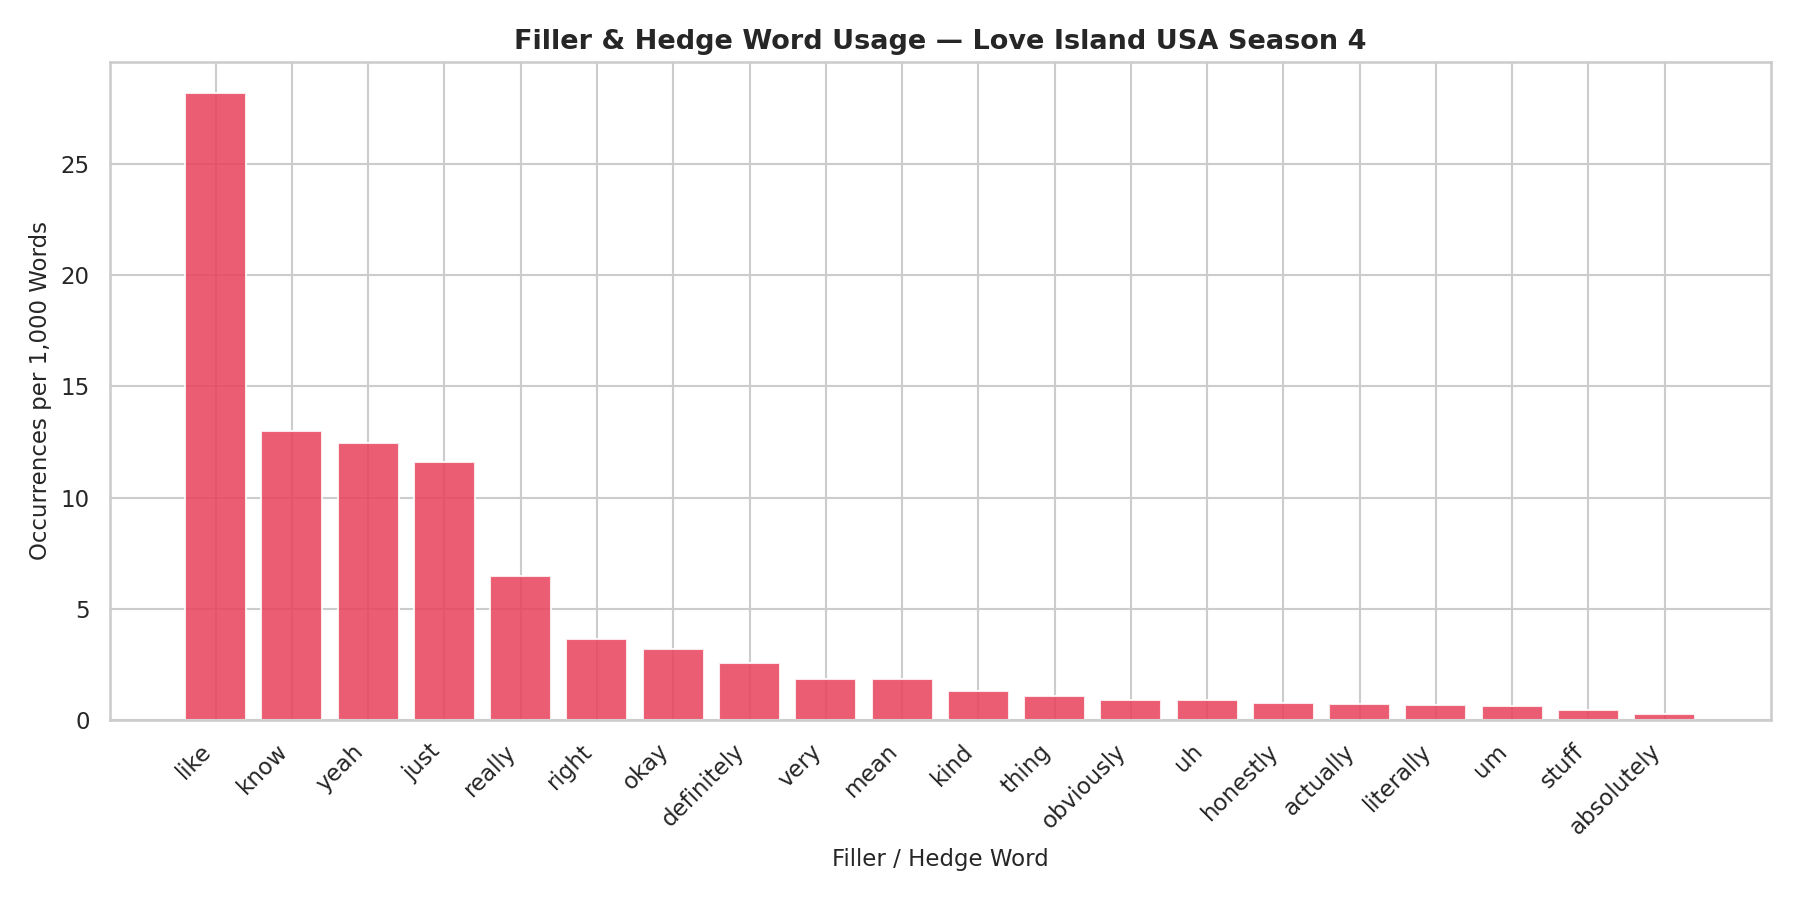
\includegraphics[width=\linewidth]{06_filler_words.png}
\caption*{\textbf{Figure 6.} Filler and Hedge Word Usage}
\end{figure}

Collectively, the 24 filler and hedge words tracked in this study account for \textbf{9.3\%} of all tokens (20,828 of 224,815) --- roughly one word in eleven. This suggests that a substantial proportion of the speech serves phatic, hedging, and discourse-organising functions rather than referential communication, aligning with Fleiss's (2018) observation that reality TV speech is heavily "approximator-laden." (Because several of these items --- notably \emph{like}, \emph{right}, \emph{mean}, \emph{kind} --- are polysemous, this figure is best read as an upper bound on purely phatic usage.)

\subsection*{4.6 Part-of-Speech Distribution}

Figure 7 shows the part-of-speech distribution of a 50,000-token sample of the corpus. Verbs are the largest category (24.5\%), followed by nouns (17.9\%), prepositions (15.4\%), and pronouns (13.6\%). Pronouns and verbs together account for 38.1\% of tokens, while adjectives and adverbs combined represent only 16.8\%.

\begin{figure}[h]
\centering
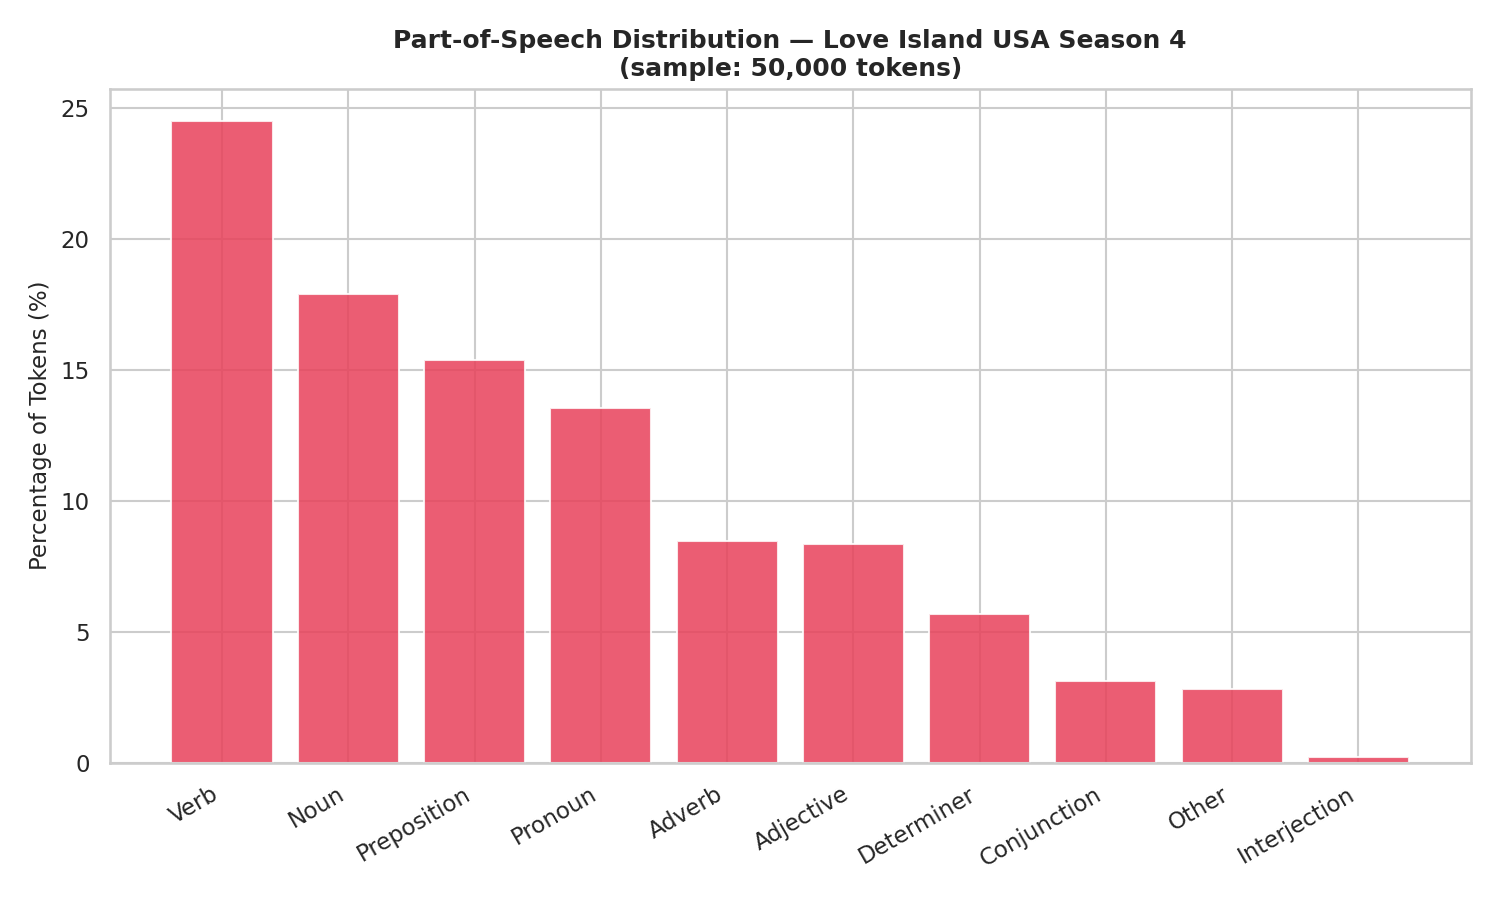
\includegraphics[width=\linewidth]{07_pos_distribution.png}
\caption*{\textbf{Figure 7.} Part-of-Speech Distribution}
\end{figure}

The relatively low proportion of adjectives (8.4\%) is particularly notable, as adjectives are a primary carrier of descriptive and evaluative meaning. The high pronoun-to-noun and verb-to-adjective ratios suggest a discourse characterised more by relational and action-oriented speech ("I want to", "you said", "we talked") than by rich descriptive elaboration. (POS tags were assigned by the NLTK averaged-perceptron tagger over lowercased, individually-listed tokens; tagger accuracy on informal, punctuation-stripped speech is lower than on edited prose, so these proportions are indicative rather than exact.)

\subsection*{4.7 Sentiment Across Episodes}

Figure 8 displays sentiment polarity and subjectivity scores per episode. Polarity scores range from 0.089 (Episode 18) to 0.278 (Episode 37), with an overall mean of 0.174. Every one of the 38 episodes scores positively on polarity, with none approaching neutrality, let alone negativity. This uniform positivity may reflect the show's emphasis on romantic pursuit and the tendency of contestants to frame experiences constructively in confessional-style speech, though it may also partly be an artefact of TextBlob's lexicon over-weighting common positive terms in casual speech (see Limitations).

\begin{figure}[h]
\centering
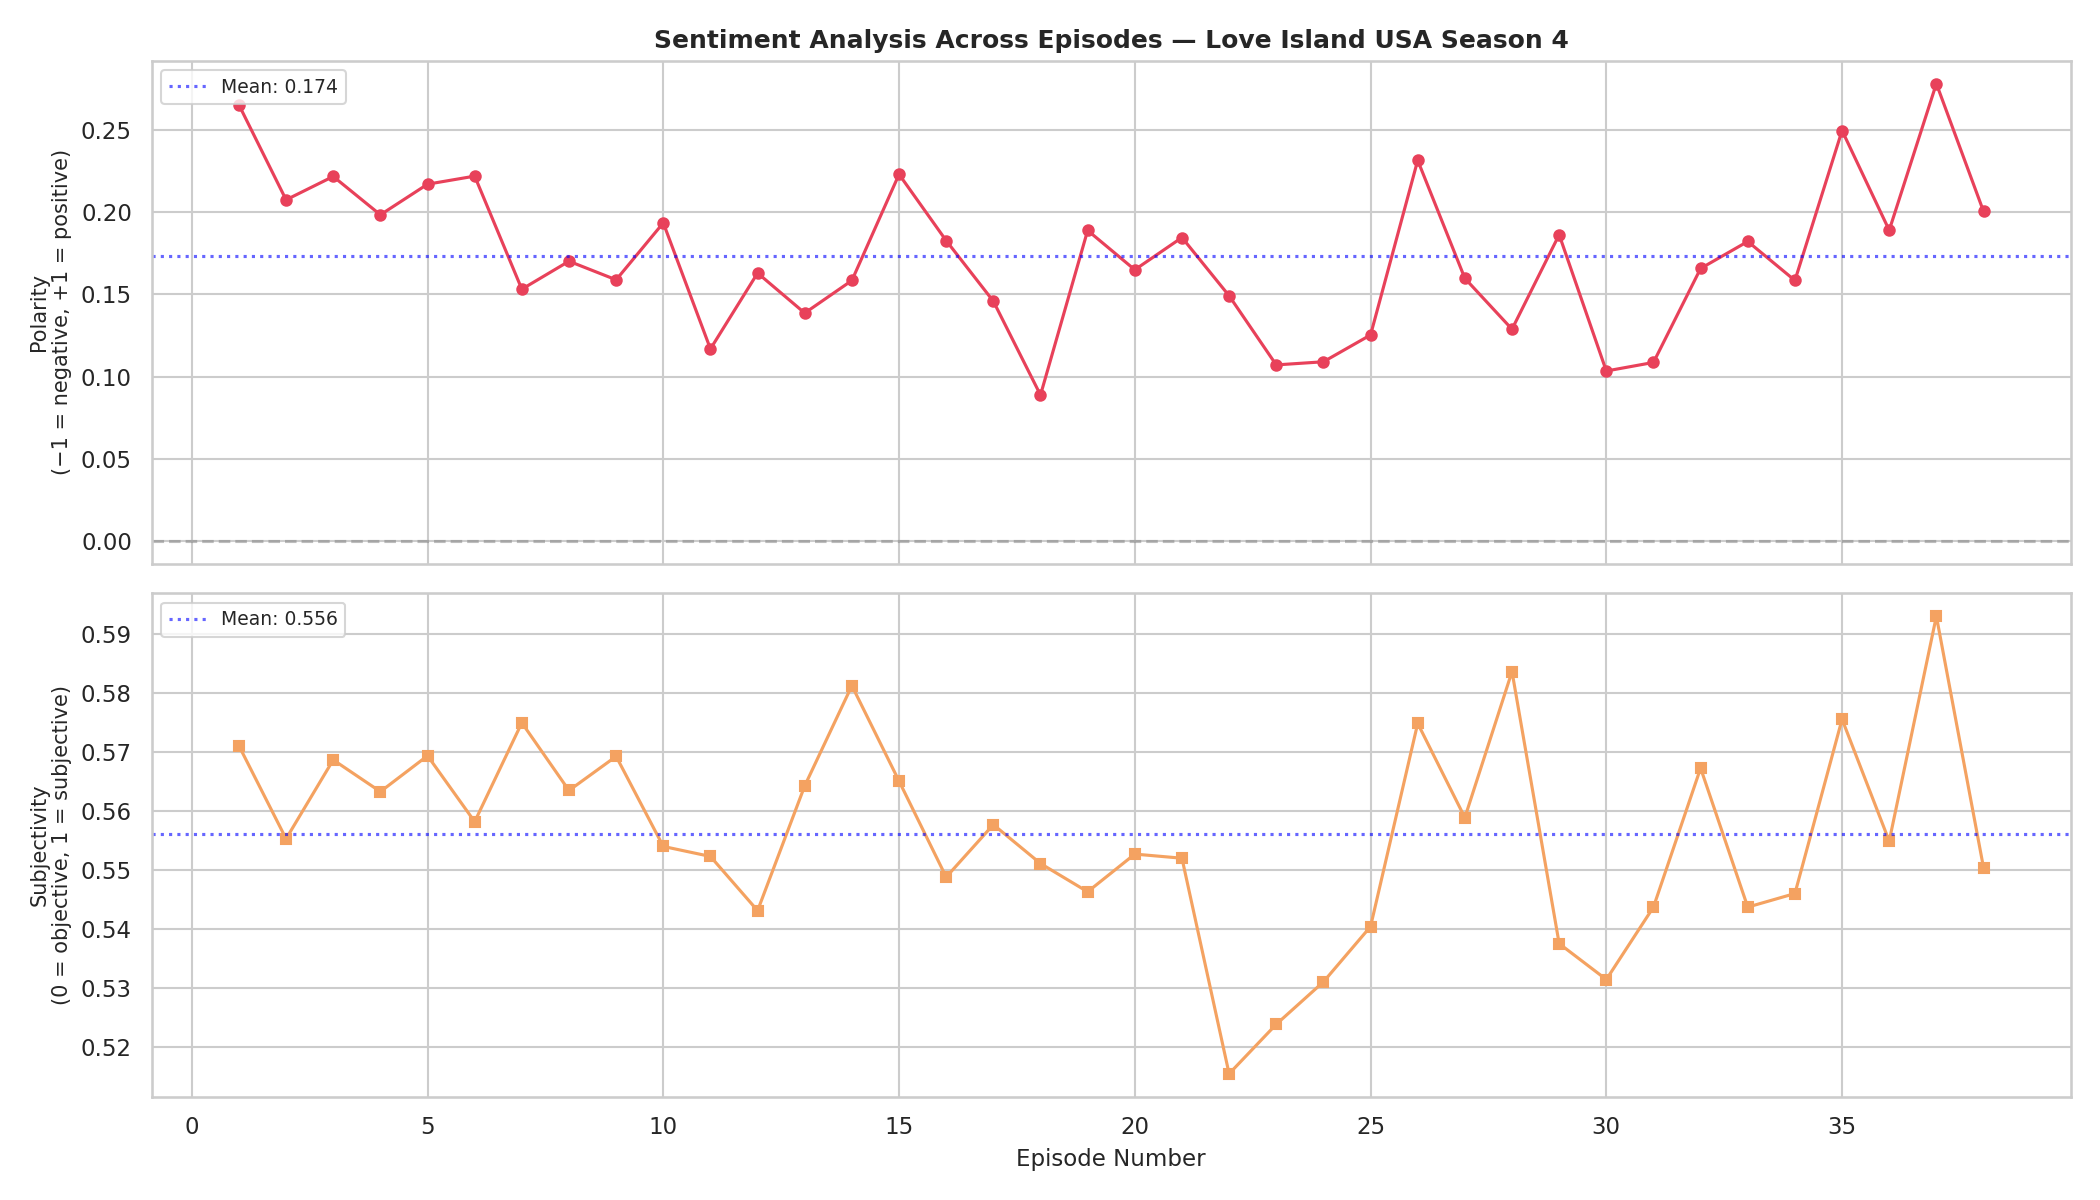
\includegraphics[width=\linewidth]{08_sentiment_per_episode.png}
\caption*{\textbf{Figure 8.} Sentiment Analysis Across Episodes}
\end{figure}

Subjectivity scores are consistently high and remarkably stable (mean 0.556, range 0.515--0.593), confirming the heavily opinion- and feeling-based nature of the discourse. The five lowest-polarity episodes (18, 30, 23, 31, 24) are distributed across the middle and later season rather than concentrated at a single narrative point, and across the season as a whole polarity shows no significant linear trend (r = $-$0.13, p = .44). Mapping these dips onto specific on-screen events (recouplings, eliminations, confrontations) would require episode-level event coding, which is left to future work.

\subsection*{4.8 Word Length Distribution}

Figure 9 shows the distribution of word lengths across the corpus. The modal word length is 4 characters (28.7\% of all tokens), and 72.9\% of all words are 1--4 characters long. The distribution falls away steeply thereafter: five-character words make up 10.1\% of tokens, and only 17.0\% are six characters or longer.

\begin{figure}[h]
\centering
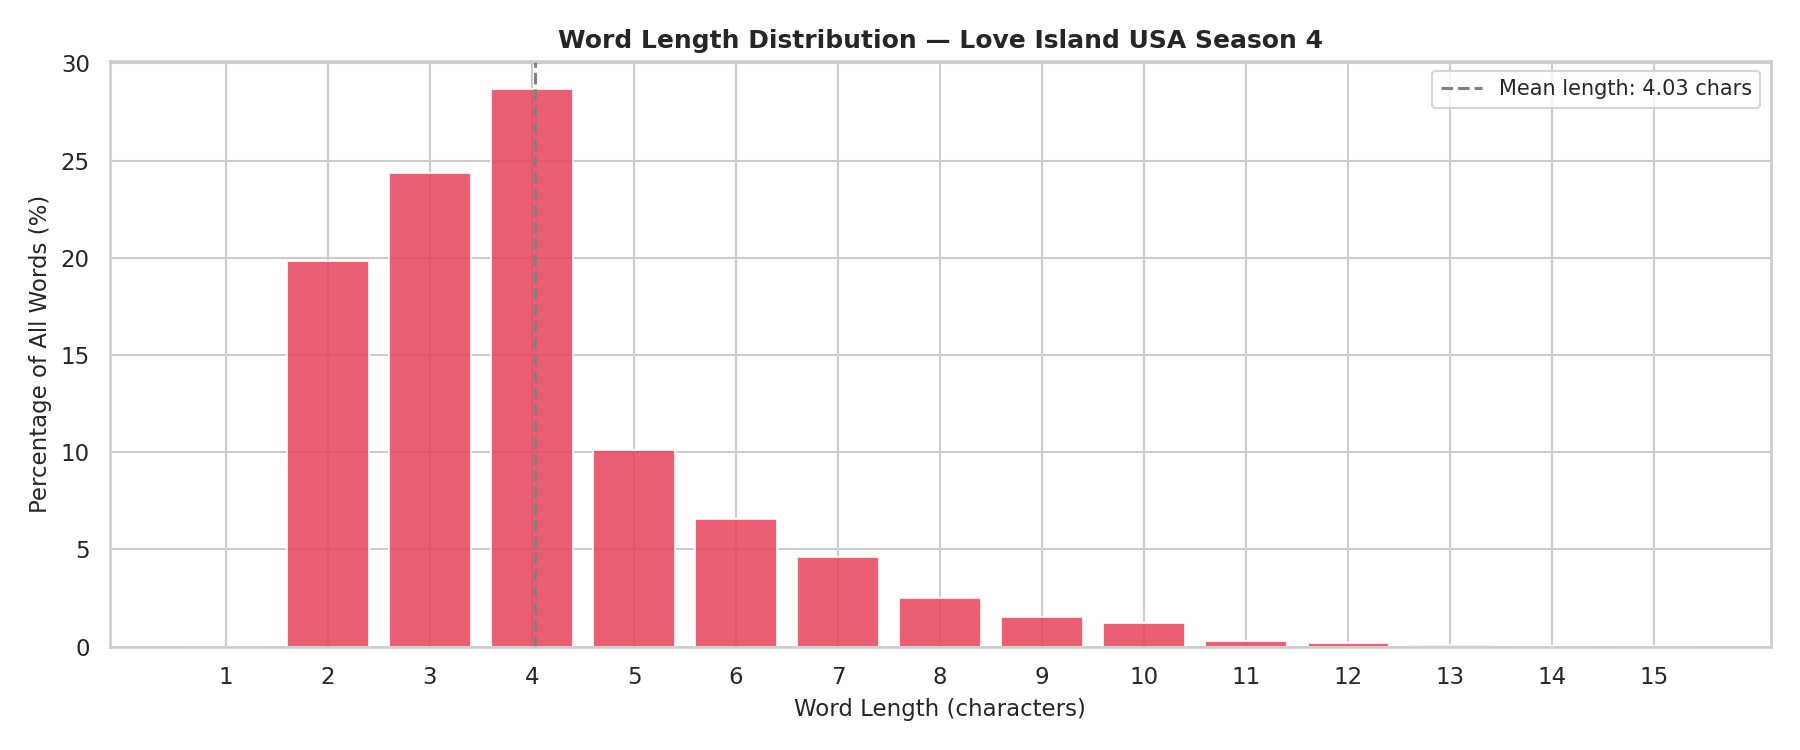
\includegraphics[width=\linewidth]{09_word_length_distribution.png}
\caption*{\textbf{Figure 9.} Word Length Distribution}
\end{figure}

The mean word length of 4.03 characters is consistent with spoken informal English, which skews shorter than written English (mean $\sim$5.1 characters in formal written corpora; Biber et al., 1999). (Note that this figure is slightly deflated by the removal of single-character tokens, which would otherwise add a one-character bar; the qualitative skew toward short words is unaffected.)

\subsection*{4.9 Vocabulary Growth Curve}

Figure 10 plots cumulative unique word types against cumulative tokens across the season. The curve shows rapid initial growth followed by gradual flattening, indicating vocabulary saturation --- most new vocabulary types are introduced early, with later episodes contributing diminishing numbers of new words. By the corpus midpoint ($\approx$112,000 tokens) 69.4\% of the season's total vocabulary has already appeared, rising to 84.8\% by the three-quarter mark.

\begin{figure}[h]
\centering
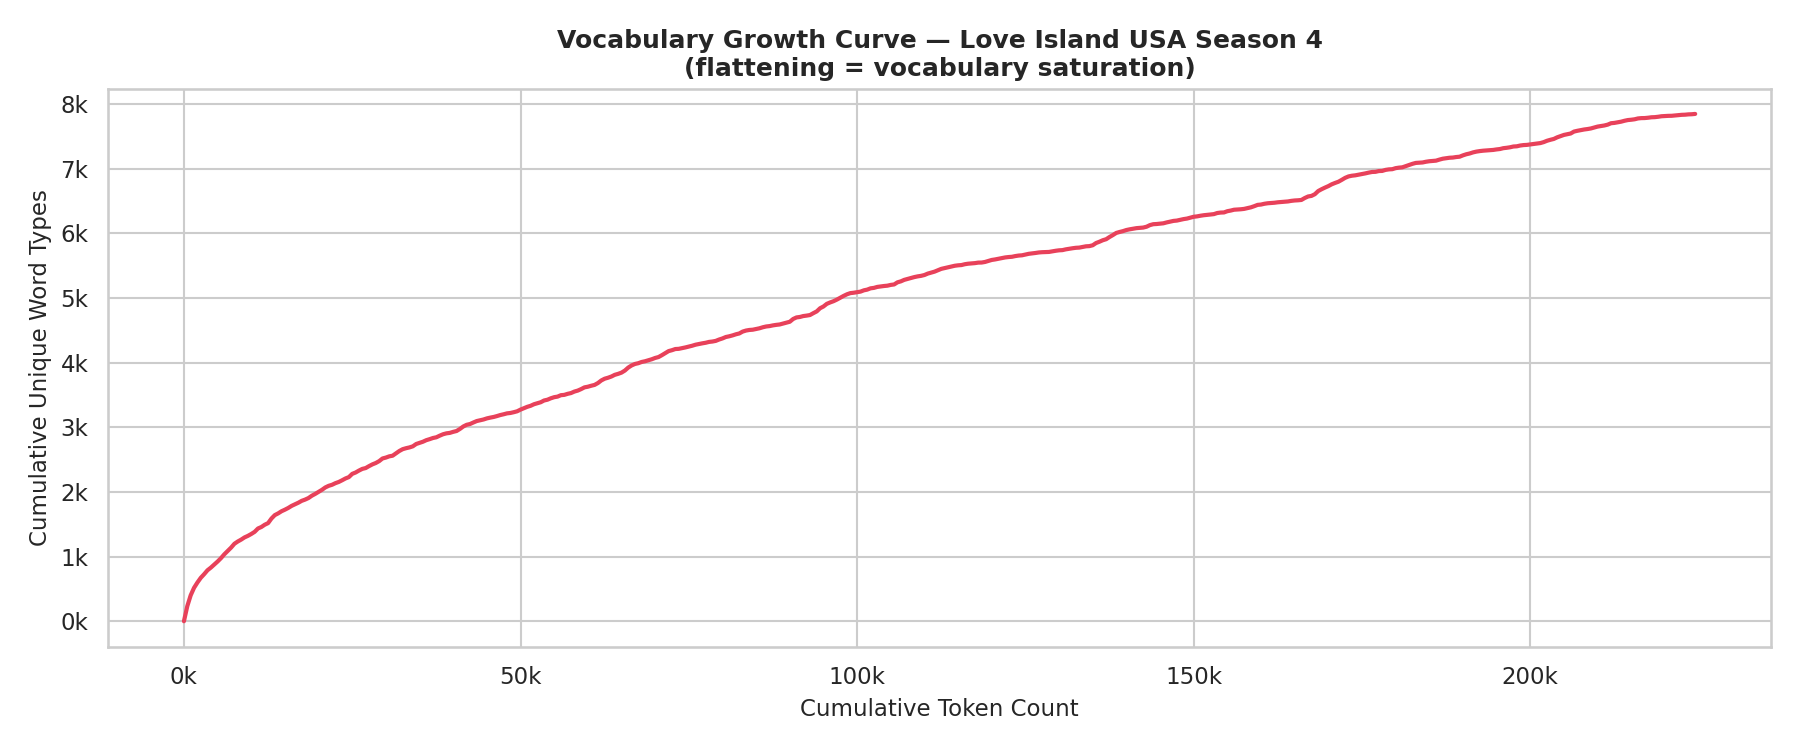
\includegraphics[width=\linewidth]{10_vocabulary_growth_curve.png}
\caption*{\textbf{Figure 10.} Vocabulary Growth Curve}
\end{figure}

Measured by episode, roughly two-thirds (67.8\%) of the season's 7,856 distinct word types have appeared by the end of Episode 19 (the season's halfway point), suggesting the show's active vocabulary is largely established within the first half of the season; the remaining episodes mostly recombine an already-settled lexicon.


\section*{5. Discussion}

\subsection*{5.1 A Constrained Vocabulary}

The results paint a consistent picture: \emph{Love Island USA} Season 4 exhibits a constrained vocabulary profile. A whole-corpus Type-Token Ratio of 0.035 and a mean per-episode MTLD of 59.96 --- below the $\approx$72 benchmark for ordinary spontaneous speech --- indicate that speakers recycle a relatively small set of words across a large volume of speech. The top 100 words account for 61\% of all tokens, just 1,000 word types cover 91\%, and the vocabulary growth curve suggests saturation is reached well before the season's end.

This is not surprising in the context of spontaneous spoken discourse, which is universally more lexically restricted than written language. However, the degree of concentration is striking, and the near-perfect Zipfian fit (R\textsuperscript{2} = 0.98) shows the distribution is highly regular rather than idiosyncratic. The dominance of discourse markers --- \emph{like} at 28.2 per 1,000 words, \emph{know} at 13.0, \emph{yeah} at 12.5 --- suggests that hedge words and discourse markers constitute a meaningful structural layer of the language, performing social rather than referential functions.

\subsection*{5.2 Emotional but Simple}

The sentiment analysis reveals a discourse that is highly subjective (mean subjectivity = 0.556) and uniformly positive in polarity, with the softest episodes (lowest polarity $\approx$ 0.09) still falling well on the positive side of the scale. This emotional texture is conveyed, paradoxically, with a limited adjectival vocabulary (just 8.4\% of tokens). Rather than deploying diverse descriptive language, speakers tend to rely on intensifiers (\emph{really}, \emph{so}) paired with a small set of high-frequency evaluative adjectives (\emph{good}, \emph{amazing}, \emph{crazy}). Emotional content, in other words, is carried more by volitional and relational verbs (\emph{feel}, \emph{love}, \emph{want}, \emph{think}) than by descriptive elaboration.

This pattern is consistent with what Biber et al. (1999) describe as "involved production" --- language produced under real-time cognitive pressure that foregrounds personal stance and interpersonal engagement over lexical elaboration.

\subsection*{5.3 Implications}

These findings carry several implications. For media and linguistics researchers, they confirm that reality TV of this type functions as a distinctive register --- one that may differ meaningfully from other forms of television discourse, and warrants further comparative study. For educators and audiences, they raise questions about whether heavy consumption of such content constitutes rich language exposure. With a core of roughly 1,000 word types accounting for 91\% of all discourse, viewers are repeatedly exposed to a narrow linguistic range.

A natural next step would be a controlled comparison with scripted television (e.g., \emph{How I Met Your Mother}, which shares a romantic thematic focus), which would allow us to isolate the effect of scripting on lexical richness.

\subsection*{5.4 Limitations}

Several limitations should be acknowledged.

\textbf{Speaker attribution.} The most important constraint is that the source subtitles carry no speaker labels. The corpus therefore mixes contestant dialogue with host/narrator commentary and voiceover, and---because contestants also enter and exit the villa throughout the season---represents many different speakers pooled together. Claims about "the language of the villa" should be read as claims about the broadcast discourse as a whole, not about any individual or about contestants in isolation. Speaker-diarised transcripts would be required to separate these voices and to support individual-level analysis.

\textbf{Transcription quality.} The transcripts are caption-derived and may contain errors, particularly with overlapping speech, proper names, and slang; informal contractions such as \emph{gonna} and \emph{wanna} are also split by the tokeniser into fragments (e.g., \emph{gon}/\emph{na}), which can inflate the apparent frequency of non-word tokens.

\textbf{Preprocessing artefacts.} Single-character tokens (\emph{I}, \emph{a}) were removed, so the single most frequent English pronoun is absent from all counts, and the mean word length is marginally deflated. These choices are documented in §3.2 and do not affect the qualitative findings, but they should be borne in mind when comparing figures to other corpora.

\textbf{Tool validity.} TextBlob's sentiment analysis is a lexicon-based method not optimised for informal, ironic, or slang-heavy speech, so the uniformly positive polarity scores may partly reflect lexicon bias rather than genuine affect; they are best treated as relative, within-corpus comparisons. Likewise, automatic POS tagging is less accurate on lowercased, punctuation-stripped conversational text than on edited prose, so the part-of-speech proportions are indicative rather than exact.

\textbf{Construct validity.} Finally, TTR and even MTLD capture vocabulary \emph{spread} but not vocabulary \emph{depth} --- knowing that a word was used does not tell us how precisely, creatively, or appropriately it was deployed. A fuller picture would combine these measures with collocational and semantic analysis.


\section*{6. Conclusion}

This study provides the first corpus-based lexical analysis of \emph{Love Island USA} Season 4. Across 224,815 word tokens drawn from 38 episodes, we find a discourse characterised by limited lexical diversity (corpus TTR: 0.035; mean MTLD: 59.96, below the $\approx$72 benchmark for spontaneous speech), heavy reliance on a small core of high-frequency words (the top 100 cover 61\% of all tokens, in near-perfect accordance with Zipf's Law), prominent use of filler and hedge language (9.3\% of tokens), and a strongly subjective, uniformly positive emotional register.

The language of the villa is expressive, relational, and emotionally immediate --- but it is not lexically varied. Whether this reflects the natural properties of unscripted emotional speech, the demographics of participants, or the communicative demands of a competitive social environment is a question for future research.

What is clear is that \emph{Love Island}, like many reality formats, presents its audience with a consistent, repetitive linguistic world --- one where the words \emph{like}, \emph{literally}, \emph{connection}, and \emph{feel} do an enormous amount of heavy lifting.


\section*{References}

Biber, D., Johansson, S., Leech, G., Conrad, S., \& Finegan, E. (1999). \emph{Longman grammar of spoken and written English}. Pearson.

Channell, J. (1994). \emph{Vague language}. Oxford University Press.

Fleiss, R. (2018). Vague language in reality television: Hedging as social performance. \emph{Journal of Sociolinguistics, 22}(3), 301--324.

Leech, G. (2000). Grammars of spoken English: New outcomes of corpus-oriented research. \emph{Language Learning, 50}(4), 675--724.

McCarthy, P. M., \& Jarvis, S. (2010). MTLD, vocd-D, and HD-D: A validation study of sophisticated approaches to lexical diversity assessment. \emph{Behavior Research Methods, 42}(2), 381--392.

Nation, I. S. P. (2001). \emph{Learning vocabulary in another language}. Cambridge University Press.

Richards, B. (1987). Type/token ratios: What do they really tell us? \emph{Journal of Child Language, 14}(2), 201--209.

Thornborrow, J., \& Morris, D. (2004). Gossip as strategy: The management of talk about others on reality TV show \emph{Big Brother}. \emph{Journal of Sociolinguistics, 8}(2), 246--271.


\section*{Appendix A --- Corpus Statistics by Episode}

\emph{Source: \texttt{output/tables/lexical\_diversity.csv}. Tokens = post-cleaning token count; Types = unique word types.}

\small\setlength{\tabcolsep}{4pt}

\begin{longtable}{llllll}
\toprule
Ep & Tokens & Types & TTR & Root TTR & MTLD \\
\midrule
\endfirsthead
\toprule
Ep & Tokens & Types & TTR & Root TTR & MTLD \\
\midrule
\endhead
\bottomrule
\endlastfoot
1 & 8650 & 1273 & 0.1472 & 13.687 & 59.21 \\
2 & 7062 & 1108 & 0.1569 & 13.185 & 43.24 \\
3 & 5930 & 995 & 0.1678 & 12.921 & 61.9 \\
4 & 5722 & 936 & 0.1636 & 12.374 & 53.98 \\
5 & 5415 & 1158 & 0.2139 & 15.737 & 81.93 \\
6 & 5317 & 920 & 0.173 & 12.617 & 62.15 \\
7 & 5447 & 953 & 0.175 & 12.913 & 59.85 \\
8 & 6468 & 950 & 0.1469 & 11.812 & 56.49 \\
9 & 5038 & 956 & 0.1898 & 13.469 & 67.12 \\
10 & 6087 & 1009 & 0.1658 & 12.933 & 55.08 \\
11 & 5961 & 1259 & 0.2112 & 16.307 & 62.39 \\
12 & 5009 & 998 & 0.1992 & 14.101 & 65.01 \\
13 & 5411 & 887 & 0.1639 & 12.058 & 54.69 \\
14 & 4750 & 918 & 0.1933 & 13.32 & 63.41 \\
15 & 5368 & 922 & 0.1718 & 12.584 & 51.89 \\
16 & 5275 & 997 & 0.189 & 13.727 & 54.35 \\
17 & 5407 & 1276 & 0.236 & 17.353 & 64.92 \\
18 & 5249 & 910 & 0.1734 & 12.56 & 76.77 \\
19 & 5176 & 996 & 0.1924 & 13.844 & 71.49 \\
20 & 5973 & 1076 & 0.1801 & 13.922 & 60.86 \\
21 & 6031 & 961 & 0.1593 & 12.375 & 59.93 \\
22 & 8294 & 1130 & 0.1362 & 12.408 & 55.45 \\
23 & 5656 & 910 & 0.1609 & 12.1 & 64.5 \\
24 & 6174 & 1227 & 0.1987 & 15.616 & 60.16 \\
25 & 5171 & 947 & 0.1831 & 13.169 & 58.74 \\
26 & 5617 & 979 & 0.1743 & 13.063 & 64.88 \\
27 & 6337 & 1032 & 0.1629 & 12.964 & 53.28 \\
28 & 4675 & 896 & 0.1917 & 13.104 & 67.98 \\
29 & 4883 & 909 & 0.1862 & 13.008 & 56.19 \\
30 & 5244 & 1286 & 0.2452 & 17.759 & 55.98 \\
31 & 5959 & 970 & 0.1628 & 12.566 & 55.62 \\
32 & 5167 & 983 & 0.1902 & 13.675 & 61.26 \\
33 & 4790 & 920 & 0.1921 & 13.293 & 54.69 \\
34 & 4763 & 923 & 0.1938 & 13.374 & 61.5 \\
35 & 7932 & 1044 & 0.1316 & 11.722 & 43.82 \\
36 & 6007 & 1240 & 0.2064 & 15.999 & 40.42 \\
37 & 6034 & 1068 & 0.177 & 13.749 & 67.58 \\
38 & 11366 & 1415 & 0.1245 & 13.272 & 69.8 \\
\end{longtable}
\normalsize\setlength{\tabcolsep}{6pt}

\section*{Appendix B --- Top 100 Words}

\emph{Source: \texttt{output/tables/top100\_words.csv}. Single-character tokens (e.g., }I\emph{, }a\emph{) excluded by preprocessing. Note the appearance of contestant first names (Isaiah, Timmy, Sydney, Deb), informal markers (bro), and tokeniser fragments of contractions (na ← gonna/wanna, gon ← gonna) within the high-frequency band.}

\small\setlength{\tabcolsep}{4pt}

\begin{longtable}{lllllllll}
\toprule
Rank & Word & Count & \% &  & Rank & Word & Count & \% \\
\midrule
\endfirsthead
\toprule
Rank & Word & Count & \% &  & Rank & Word & Count & \% \\
\midrule
\endhead
\bottomrule
\endlastfoot
1 & you & 9228 & 4.105 &  & 51 & did & 815 & 0.363 \\
2 & to & 6545 & 2.911 &  & 52 & go & 814 & 0.362 \\
3 & like & 6338 & 2.819 &  & 53 & at & 809 & 0.36 \\
4 & the & 5972 & 2.656 &  & 54 & get & 806 & 0.359 \\
5 & and & 5289 & 2.353 &  & 55 & they & 805 & 0.358 \\
6 & it & 4684 & 2.083 &  & 56 & her & 803 & 0.357 \\
7 & that & 4592 & 2.043 &  & 57 & one & 793 & 0.353 \\
8 & know & 2920 & 1.299 &  & 58 & out & 751 & 0.334 \\
9 & yeah & 2802 & 1.246 &  & 59 & shit & 731 & 0.325 \\
10 & do & 2702 & 1.202 &  & 60 & okay & 715 & 0.318 \\
11 & just & 2604 & 1.158 &  & 61 & now & 702 & 0.312 \\
12 & is & 2595 & 1.154 &  & 62 & if & 693 & 0.308 \\
13 & so & 2408 & 1.071 &  & 63 & would & 690 & 0.307 \\
14 & in & 2299 & 1.023 &  & 64 & can & 680 & 0.302 \\
15 & of & 2244 & 0.998 &  & 65 & bro & 674 & 0.3 \\
16 & me & 2182 & 0.971 &  & 66 & him & 633 & 0.282 \\
17 & was & 2100 & 0.934 &  & 67 & see & 625 & 0.278 \\
18 & for & 2083 & 0.927 &  & 68 & gon & 595 & 0.265 \\
19 & with & 2061 & 0.917 &  & 69 & definitely & 570 & 0.254 \\
20 & we & 2036 & 0.906 &  & 70 & time & 565 & 0.251 \\
21 & what & 1978 & 0.88 &  & 71 & because & 563 & 0.25 \\
22 & my & 1962 & 0.873 &  & 72 & back & 557 & 0.248 \\
23 & this & 1570 & 0.698 &  & 73 & island & 515 & 0.229 \\
24 & have & 1556 & 0.692 &  & 74 & been & 509 & 0.226 \\
25 & be & 1510 & 0.672 &  & 75 & let & 502 & 0.223 \\
26 & on & 1505 & 0.669 &  & 76 & girl & 501 & 0.223 \\
27 & he & 1482 & 0.659 &  & 77 & who & 498 & 0.222 \\
28 & really & 1456 & 0.648 &  & 78 & man & 493 & 0.219 \\
29 & but & 1404 & 0.625 &  & 79 & little & 486 & 0.216 \\
30 & oh & 1382 & 0.615 &  & 80 & more & 478 & 0.213 \\
31 & are & 1369 & 0.609 &  & 81 & as & 461 & 0.205 \\
32 & up & 1210 & 0.538 &  & 82 & from & 444 & 0.197 \\
33 & all & 1194 & 0.531 &  & 83 & when & 440 & 0.196 \\
34 & feel & 1174 & 0.522 &  & 84 & had & 434 & 0.193 \\
35 & love & 1137 & 0.506 &  & 85 & look & 432 & 0.192 \\
36 & not & 1128 & 0.502 &  & 86 & say & 431 & 0.192 \\
37 & she & 1101 & 0.49 &  & 87 & or & 430 & 0.191 \\
38 & good & 1079 & 0.48 &  & 88 & isaiah & 427 & 0.19 \\
39 & think & 1035 & 0.46 &  & 89 & timmy & 424 & 0.189 \\
40 & about & 938 & 0.417 &  & 90 & very & 417 & 0.185 \\
41 & how & 938 & 0.417 &  & 91 & mean & 416 & 0.185 \\
42 & your & 924 & 0.411 &  & 92 & too & 408 & 0.181 \\
43 & na & 906 & 0.403 &  & 93 & come & 401 & 0.178 \\
44 & there & 906 & 0.403 &  & 94 & fuck & 398 & 0.177 \\
45 & want & 851 & 0.379 &  & 95 & sydney & 397 & 0.177 \\
46 & here & 842 & 0.375 &  & 96 & deb & 396 & 0.176 \\
47 & got & 837 & 0.372 &  & 97 & fucking & 387 & 0.172 \\
48 & going & 818 & 0.364 &  & 98 & will & 386 & 0.172 \\
49 & right & 817 & 0.363 &  & 99 & well & 382 & 0.17 \\
50 & no & 815 & 0.363 &  & 100 & make & 381 & 0.169 \\
\end{longtable}
\normalsize\setlength{\tabcolsep}{6pt}

\section*{Appendix C --- Filler Word Frequencies}

\emph{Source: \texttt{output/tables/filler\_word\_counts.csv}. Per-1,000 and \% computed over 224,815 tokens.}

\small\setlength{\tabcolsep}{4pt}

\begin{longtable}{llll}
\toprule
Filler word & Count & Per 1,000 words & \% of total \\
\midrule
\endfirsthead
\toprule
Filler word & Count & Per 1,000 words & \% of total \\
\midrule
\endhead
\bottomrule
\endlastfoot
like & 6338 & 28.19 & 2.819 \\
know & 2920 & 12.99 & 1.299 \\
yeah & 2802 & 12.46 & 1.246 \\
just & 2604 & 11.58 & 1.158 \\
really & 1456 & 6.48 & 0.648 \\
right & 817 & 3.63 & 0.363 \\
okay & 715 & 3.18 & 0.318 \\
definitely & 570 & 2.54 & 0.254 \\
very & 417 & 1.85 & 0.185 \\
mean & 416 & 1.85 & 0.185 \\
kind & 292 & 1.3 & 0.13 \\
thing & 242 & 1.08 & 0.108 \\
obviously & 201 & 0.89 & 0.089 \\
uh & 201 & 0.89 & 0.089 \\
honestly & 171 & 0.76 & 0.076 \\
actually & 162 & 0.72 & 0.072 \\
literally & 153 & 0.68 & 0.068 \\
um & 140 & 0.62 & 0.062 \\
stuff & 99 & 0.44 & 0.044 \\
absolutely & 57 & 0.25 & 0.025 \\
basically & 22 & 0.1 & 0.01 \\
seriously & 14 & 0.06 & 0.006 \\
sort & 10 & 0.04 & 0.004 \\
totally & 9 & 0.04 & 0.004 \\
\end{longtable}
\normalsize\setlength{\tabcolsep}{6pt}

\section*{Appendix D --- Sentiment Scores by Episode}

\emph{Source: \texttt{output/tables/sentiment\_scores.csv}. TextBlob polarity ($-$1 to +1) and subjectivity (0 to 1), computed over full episode text.}

\small\setlength{\tabcolsep}{4pt}

\begin{longtable}{lll}
\toprule
Ep & Polarity & Subjectivity \\
\midrule
\endfirsthead
\toprule
Ep & Polarity & Subjectivity \\
\midrule
\endhead
\bottomrule
\endlastfoot
1 & 0.2651 & 0.5711 \\
2 & 0.2074 & 0.5553 \\
3 & 0.2216 & 0.5687 \\
4 & 0.1983 & 0.5633 \\
5 & 0.2169 & 0.5694 \\
6 & 0.2218 & 0.5582 \\
7 & 0.1531 & 0.575 \\
8 & 0.1701 & 0.5635 \\
9 & 0.1588 & 0.5693 \\
10 & 0.1934 & 0.554 \\
11 & 0.1168 & 0.5523 \\
12 & 0.1629 & 0.5431 \\
13 & 0.1386 & 0.5643 \\
14 & 0.1584 & 0.5813 \\
15 & 0.2229 & 0.5651 \\
16 & 0.1826 & 0.5488 \\
17 & 0.1458 & 0.5577 \\
18 & 0.0888 & 0.5511 \\
19 & 0.1888 & 0.5463 \\
20 & 0.1649 & 0.5527 \\
21 & 0.1845 & 0.552 \\
22 & 0.1491 & 0.5154 \\
23 & 0.1071 & 0.5238 \\
24 & 0.109 & 0.531 \\
25 & 0.1253 & 0.5404 \\
26 & 0.2314 & 0.5749 \\
27 & 0.1597 & 0.5589 \\
28 & 0.1288 & 0.5837 \\
29 & 0.1862 & 0.5375 \\
30 & 0.1034 & 0.5314 \\
31 & 0.1086 & 0.5437 \\
32 & 0.1657 & 0.5673 \\
33 & 0.1821 & 0.5437 \\
34 & 0.1584 & 0.546 \\
35 & 0.2495 & 0.5756 \\
36 & 0.1889 & 0.5549 \\
37 & 0.278 & 0.5931 \\
38 & 0.2004 & 0.5504 \\
\end{longtable}
\normalsize\setlength{\tabcolsep}{6pt}

\section*{Appendix E --- Statistical Tests}

\emph{Source: \texttt{output/tables/statistical\_tests.csv}. Trend correlations are across the 38 episodes (n = 38); Zipf regression is over all ranked word types.}

\begin{longtable}{p{0.78\linewidth}ll}
\toprule
Test & Statistic & p-value \\
\midrule
\endfirsthead
\toprule
Test & Statistic & p-value \\
\midrule
\endhead
\bottomrule
\endlastfoot
Cumulative \% of tokens --- top 10 words & 22.72\% & --- \\
Cumulative \% of tokens --- top 50 words & 48.71\% & --- \\
Cumulative \% of tokens --- top 100 words & 61.02\% & --- \\
Cumulative \% of tokens --- top 1,000 words & 91.11\% & --- \\
Zipf regression slope (log freq $\sim$ log rank) & $-$1.453 & $<$ .001 \\
Zipf regression R\textsuperscript{2} & 0.981 & --- \\
MTLD vs. episode --- Pearson r & $-$0.107 & .521 \\
MTLD vs. episode --- Spearman $\rho$ & $-$0.028 & .868 \\
TTR vs. episode --- Pearson r & 0.048 & .775 \\
TTR vs. episode --- Spearman $\rho$ & 0.109 & .514 \\
Sentiment polarity vs. episode --- Pearson r & $-$0.129 & .441 \\
Sentiment polarity vs. episode --- Spearman $\rho$ & $-$0.149 & .371 \\
\end{longtable}


\emph{Analysis performed using Python 3.12 (\texttt{nltk}, \texttt{textblob}, \texttt{scipy}, \texttt{wordcloud}, \texttt{pandas}, \texttt{matplotlib}, \texttt{seaborn}). Scripts (\texttt{analyze\_love\_island.py}), the cleaned corpus (\texttt{love\_island\_s4\_transcripts.csv}), and all output tables and figures are available on request.}

\end{document}
